\documentclass[a4paper,11pt]{article}
\usepackage{ifpdf}
\ifpdf
  \usepackage[pdftex]{graphicx}
  \DeclareGraphicsExtensions{.mps,.pdf,.jpg,.png}%
  \DeclareGraphicsRule{*}{mps}{*}{}
\else
  \usepackage[dvips]{graphicx}
  \DeclareGraphicsExtensions{.mps,.eps}%
  \DeclareGraphicsRule{*}{eps}{*}{}
\fi

\usepackage{amsmath,amssymb}
\usepackage{amsthm}

\newtheorem{lemma}{Lemma}
\newtheorem{corollary}{Corollary}
\newtheorem{theorem}{Theorem}
\newtheorem{acknowledgement}[theorem]{Acknowledgement}
\newtheorem{algorithm}[theorem]{Algorithm}
\newtheorem{axiom}[theorem]{Axiom}
\newtheorem{case}[theorem]{Case}
\newtheorem{claim}[theorem]{Claim}
\newtheorem{conclusion}[theorem]{Conclusion}
\newtheorem{condition}[theorem]{Condition}
\newtheorem{conjecture}[theorem]{Conjecture}
\newtheorem{criterion}[theorem]{Criterion}
\newtheorem{definition}[theorem]{Definition}
\newtheorem{example}[theorem]{Example}
\newtheorem{exercise}[theorem]{Exercise}
\newtheorem{notation}[theorem]{Notation}
\newtheorem{problem}[theorem]{Problem}
\newtheorem{proposition}[theorem]{Proposition}
\newtheorem{remark}[theorem]{Remark}
\newtheorem{solution}[theorem]{Solution}
\newtheorem{summary}[theorem]{Summary}

\usepackage{bm}

\providecommand{\abs}[1]{\left\lvert#1\right\rvert}
\renewcommand{\phi}{\varphi}
\renewcommand{\Phi}{\varPhi}
\renewcommand{\Gamma}{\varGamma}
\renewcommand{\Lambda}{\varLambda}
%\renewcommand{\Omega}{\varOmega}
\renewcommand{\Re}{\operatorname{Re}}
\renewcommand{\Im}{\operatorname{Im}}
\renewcommand{\vec}[1]{\bm{#1}}
\renewcommand{\i}{\,\mathrm{i}}
\newcommand{\e}{\,\mathrm{e}}
\newcommand{\scl}{Schwarz--Chris\-tof\-fel}
\newcommand{\scm}{Schwarz--Chris\-tof\-fel mapping}
\newcommand{\upl}{\Pi^+}
\newcommand{\uplc}{\overline{\Pi}\,^+}
\newcommand{\R}{\mathbb R}
\newcommand{\C}{\mathbb C}
\newcommand{\cf}{\mathcal{C}}
\newcommand{\imp}{\Rightarrow}
\newcommand{\pd}[2]{\dfrac{\partial#1}{\partial#2}}
\newcommand{\pdt}[2]{\partial#1/\partial#2}
\newcommand{\du}{\pd{}u}
\newcommand{\ddu}{\pd{{}^2}{u^2}}
\renewcommand{\Lambda}{\varLambda}
\renewcommand{\Delta}{\varDelta}
\newcommand{\Lp}{\Lambda^+(u,u_2)}
\newcommand{\Dp}{\Delta^+(u,u_2)}
\newcommand{\Rp}{R^+(u,u_2)}
\newcommand{\Tp}{T^+(u,u_2)}
\renewcommand{\Phi}{\varPhi}
\newcommand{\Phip}{\vec\Phi^+}
\newcommand{\Phim}{\vec\Phi^-}
\newcommand{\Phiin}{\vec\Phi^{\text{in}}}
\newcommand{\ms}{\hphantom{-}}
\newcommand{\Ttot}{T^+_{\text{tot}}}
\newcommand{\Rtot}{R^+_{\text{tot}}}

\begin{document}


\title{Fourier Methods for Harmonic Scalar Waves in General
  Waveguides}

\author{Anders Andersson, B\"orje Nilsson, Thomas Biro}
\maketitle

\section{Introduction}
\label{sec:intro}

Wave scattering in waveguides of different shapes is a classical
problem in applied mathematics. The problem appears in many
applications, in acoustics, optics, electro-dynamics and quantum
physics.

When treating this problem mathematically, the task is to find
solutions to the wave equation in some of its forms, and an essential
part of this task is to solve Helmholtz equation
\begin{equation}
  \label{eq:Helmholtz1}
  (\nabla^2+k^2)p=0
\end{equation}
in different geometries and with various boundary conditions.

For simple geometries, for example straight channels with hard or soft
walls, the solutions are easily found in terms of Fourier
series. Examples using this technique are found in any basic text on
partial differential equations. For more complex geometries or
boundary conditions, purely numerical methods or more precisely, finite
element methods, have during recent years, due to evolution of both
the methods and the computers, become the natural choice for solving
Helmholtz equation.

% However, this is not done without problems. It is a well-known fact
% that FEM-based methods run into trouble, i.e., require an extremely
% fine mesh and hence huge amounts of computer memory, in the low
% frequency domain, i.e., when the constant $k$ in
% (\ref{eq:Helmholtz1}) is small.

However, motivated by both the mathematics and applications involving
inverse wave scattering problems, we find it interesting to see what
can be done with the classical semi-analytic Fourier methods, even
when the geometries and the boundary conditions are complex.

The purpose of this article is exactly this, to investigate and to
show how Fourier methods can be used to solve wave scattering problems
in a waveguide with geometry and boundary conditions that exceed the
ordinary school book examples. To be able to do that, we use a toolbox
containing a set of methods:
\begin{itemize}
\item The Building Block Method makes it possible to divide a
  complicated geometry into several tractable parts.
\item Different conformal mapping methods are used to further simplify
  the geometry.
\item Reformulation of (\ref{eq:Helmholtz1}) assuming that the field
  can be expressed in Fourier series.
\item Determination of numerically stable differential equations for
  reflection and transmission operators means that these can be
  determined for each part of the waveguide.
\item Dirichlet-to-Neumann operators make it possible to formulate and
  solve numerically stable differential equations for the field in the
  waveguide.
\end{itemize}

Additional well-known tools such as mode matching and Wiener--Hopf
methods, are necessary to solve general waveguide problems, but are
not used in this article.

In an example taken from acoustic, i.e., the field in the waveguide
is scalar, we show how these techniques can be combined, in order to
get the complete solution of Helmholtz equation in a general
waveguide. The results in this example are then compared with the
results when using commercial finite element software to solve the
problem.

The plan of the paper is as follows: In Section~\ref{sec:prel}, the
mathematical basis for a Fourier solution is outlined and in
Section~\ref{sec:oneblock}, it is described how the field as well as
reflection and transmission operators are determined in a single
``block'', using conformal mappings and different reformulations of
equation~(\ref{eq:Helmholtz1}).  Section~\ref{sec:comb-blocks-build}
shows how these blocks can be combined, using the Building Block
Method. Section~\ref{sec:numerical-example} contains the example
problem and a detailed description of the techniques used to solve
it. Finally, some final comments are included in
Section~\ref{sec:conclusion}.

\section{Preliminaries}
\label{sec:prel}

The problem under investigation is propagation of scalar harmonic
waves in a waveguide $V$, in $\mathbb{R}^{2}$ or $\mathbb{R}^{3},$ of
rather general shape. Acoustic notation is used where the sound
pressure $p$ solves Helmholtz equation%
\begin{equation}
  (\nabla^{2}+k^{2})p(\bm{r})=0,\text{ }\bm{r}\in V\text{,} \label{101}%
\end{equation}
in the interior $V$ of the waveguide and fulfils a homogeneous
boundary condition%
\begin{equation}
  \dfrac{\partial p}{\partial n}=\text{i}k\beta p,
  \text{ }\bm{r}\in\partial V\text{,} \label{102}%
\end{equation}
on the boundary $\partial V$. Here, $k\in\mathbb{R}^{+}$ is the
wavenumber, $\beta\in\mathbb{C}$, $\Re\beta\geq0$ is the (normalised)
surface admittance and $\widehat{\bm{n}}$ is the outward pointing
normal to $\partial V$. Special cases of the boundary conditions are
$\beta=0$ (Neumann or hard) and $\beta=\i\infty$ (Dirichlet or
soft). The formulation assumes the time dependence $\exp(-\i kc_{0}t)$
in the underlying wave equation. In addition to the sound velocity
$c_{0},$ the acoustic medium in the waveguide is characterised by the
density $\rho_{0}.$ Both $c_{0}$ and $\rho_{0}$ are constant and real.

The waveguide $V$ $\subset\mathbb{R}^{n},n=2,3,$ consists of three
parts: an inner bounded and connected part $V_{\text{i}}$ and two
straight semi-infinite parts $V_{\text{L}}$ and $V_{\text{R}}$. An
axial co-ordinate $u$ is associated to the waveguide with the positive
axis aligned with $V_{\text{R}}$ and the negative with $V_{\text{L}}.$
Fig.  \ref{fig:wg1} depicts this waveguide schematically.%
\begin{figure}[htb]
  \centering
  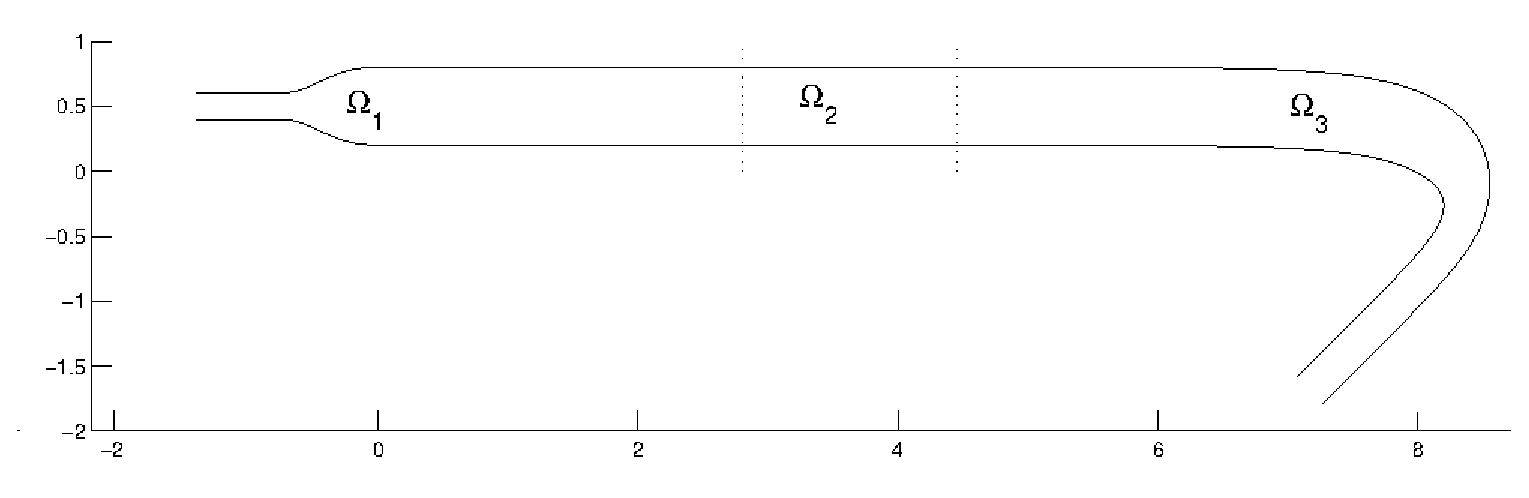
\includegraphics[scale=1]{waveguide.1}
  \caption{Waveguide $V=V_L\cup V_i\cup V_R$ consisting of straight
    parts $V_L$ and $V_R$ open to infinity and a bounded connecting
    part $V_i$.}
  \label{fig:wg1}
\end{figure}
Using the notation $\mathbb{R}_{u_0}^{\pm}=\left\{ u\in\mathbb{R}:\
  u\gtrless u_{0}\right\} ,$ the straight waveguide parts are
$V_{\text{L}%
}=\Omega_{\text{L }}\times\mathbb{R}_{u_{\text{L}}}^{-}$ and
$V_{\text{R}%
}=\Omega_{\text{R }}\times\mathbb{R}_{u_{\text{R}}}^{+},$ where
$\Omega _{\text{L }}$ and $\Omega_{\text{R }}$ are simply connected
with boundary that is piecewise of class $C^{1}.$ This means that
Green's theorem is applicable.  For simplicity it is assumed that the
surface admittance $\beta=0$ on $\partial V_{\text{L}}\cap\partial V$
and on $\partial V_{\text{R}}\cap\partial V$, whereas $\beta$ can be
non-vanishing and varying on $V_{\text{i}}.$

As a preparation for the definition of the scattering problem, we
discuss propagation of waves in an infinite straight waveguide
$V_{\text{s}}$ $=\Omega\times\mathbb{R},$ where $\Omega$ is
$\Omega_{\text{L }}$ or $\Omega_{\text{R }}.$ If $p$ solves
(\ref{101}) in $V_{\text{s}},$ $p$ can be uniquely splitted into%
\begin{equation}
  p=p_{-}+p_{+}, \label{103}%
\end{equation}
where%
\begin{equation}
  p_{\pm}=\sum_{n}p_{n}^{\pm}\text{e}^{\pm\text{i}\alpha_{n}u}\varphi
  _{n}(\bm{r}_{\perp}),\text{ }\bm{r}_{\perp}\in\Omega. \label{104}%
\end{equation}
Here, $\varphi_{n}$ and $\lambda_{n}\geq0$ are solutions to the
eigenvalue problem%
\begin{equation}
  \left\{
    \begin{array}
      [c]{l}%
      (\nabla_{\perp}^{2}+\lambda_{n}^{2})\varphi_{n}(\bm{r}_{\perp})=0,
      \text{
      }\bm{r}_{\perp}\in\Omega\\[1ex]%
      \dfrac{\partial\varphi_{n}}{\partial n}(\bm{r}_{\perp})=0,\text{
      }\bm{r}_{\perp}\in\partial\Omega\\[2ex]%
      \int_{\Omega}\varphi_{n}^{2}(\mathbf{r}_{\perp})\text{d}\Omega=1
    \end{array}
  \right.  , \label{105}%
\end{equation}
$\nabla_{\perp}^{2}$ is the restriction of the Laplace operator to
$\Omega,$ and%
\begin{equation}
  \alpha_{n}=\left\{
    \begin{array}
      [c]{l}%
      \sqrt{k^{2}-\lambda_{n}^{2}},\text{ }k\geq\lambda_{n}\\[1ex]%
      \text{i}\sqrt{\lambda_{n}^{2}-k^{2}},\text{ }k<\lambda_{n}%
    \end{array}
  \right.  . \label{106}%
\end{equation}

We are interested in a solution $p$ that has a finite (real and
virtual) acoustic power in the axial direction and define to this end
the function space%
\begin{equation}
  X_{\pm}=\left\{  p_{\pm}=%
    % TCIMACRO{\tsum _{n}}%
    % BeginExpansion
    {\textstyle\sum_{n}}
    % EndExpansion
    p_{n}^{\pm}\text{e}^{\pm\text{i}\alpha_{n}u}\varphi_{n}(\bm{r}_{\perp})
    \text{:}%
    % TCIMACRO{\tsum _{n}}%
    % BeginExpansion
    {\textstyle\sum_{n}}
    % EndExpansion
    \left\vert \alpha_{n}\right\vert
    \left\vert p_{n}^{\pm}\right\vert ^{2}%
    <\infty\right\}  \label{107}%
\end{equation}
and $X=X_{-}\oplus X_{+}.$ Then, $p_{-}\in X_{-},$ $p_{+}\in X_{+}$
and $p\in X.$

If $p_{+}\neq0,$ we say that there is a source at $u=-\infty,$
and if $p_{-}\neq0,$ there is a source at $u=+\infty.$ Assume that
there is a region $V_{0}\subset V$, containing sources, i.e.$,$ where
$(\nabla^{2}+k^{2}%
)p\neq0,$ and that this source region is confined to the interval
$u_{-}<u<u_{+}.$ In physical terms, there should be only outgoing
waves outside the source region, i.e., leftgoing to the left and
rightgoing to the right. In order to couple this requirement to our
definition of $p_{-}$ and $p_{+},$ we formulate the following

\begin{axiom}
  \label{axiom1}
\item For the solution to $(\nabla^{2}+k^{2})p=-q$ in $V_{\text{s}},$
  where $q=0$ for $u<u_{-}$ and $u>u_{+},$%
  \[
  \left.
    \begin{array} [c]{l}%
      p=p_{-},\text{ when }u<u_{-}
      \text{ and there is no source in }u=-\infty\\
      p=p_{+},\text{ when }u>u_{+}
      \text{ and there is no source in }u=+\infty
    \end{array}
  \right.  .
  \]
\end{axiom}

\begin{description}
\item[Comment 1] Axiom \ref{axiom1} makes it natural to denote $p_{-}$
  as leftgoing and $p_{+}$ as rightgoing.

\item[Comment 2] Axiom \ref{axiom1} can be derived from physical
  principles: (a) According to the principle of vanishing absorption,
  $k$ is replaced by $k+\i\varepsilon,$ $\varepsilon>0,$ requiring
  that the solution $p$ tends to zero when the distance to the source
  region tends to infinity; then the limit of vanishing $\varepsilon$
  is taken. (b) According to the principle of causality, which is a
  fundamental physical principle, asymptotic or stationary solutions
  for large $t$ to the wave equation $(\nabla^{2}-c_{0}^{-2}%
  \partial^{2}/\partial t^{2})p=-q(\bm{r})$H$(t)\sin(kc_{0}t)$ is
  studied, where H$(t)$ is Heaviside's step function. For both cases
  a) and b), Axiom \ref{axiom1} follows with $p_{\pm}$ according to
  (\ref{104}-\ref{106}).
\end{description}

% \subsection{Formulation and simplification of the scattering
% problem}

% A scattering problem consists of the determination of reflected and
% transmitted waves when sources at infinity, or equivalently incident
% waves, are known. Connecting waveguides are assumed to be straight,
% which is motivated by the sake of simplicity and by applications;
% the splitting $p=p_{-}+p_{+}$ in leftgoing and rightgoing waves is
% possible for other geometries but the theory would be more
% complicated. Let us study the waveguide depicted in
% Figure~\ref{fig:wg2} a with a wave incident from left only. Then we
% have
% \begin{equation}
%   \left\{
%     \begin{array}
%       [c]{l}%
%       p=p_{+}^{A,\text{ in}}+R^{A}p_{+}^{A,\text{ in}}\text{ in }A\\
%       p=p_{-}+p_{+}\text{ in }B\\
%       p=T^{CA}p_{+}^{A,\text{ in}}\text{ in }C
%     \end{array}
%   \right.  .\label{108}%
% \end{equation}
% Here, $p_{+}^{A,\text{ in}}$ is the known incident wave from left,
% $R^{A}$: $X_{+}^{A}\rightarrow X_{-}^{A},$ is the reflection
% operator and $T^{CA}$: $X_{+}^{A}\rightarrow X_{+}^{C},$ is the
% transmission operator. A super index $A,B,C$ indicates the specific
% waveguide. Note that the connecting region between the straight
% waveguides is assumed to be bounded.%

% \begin{figure}[htb]
%   \centering
%   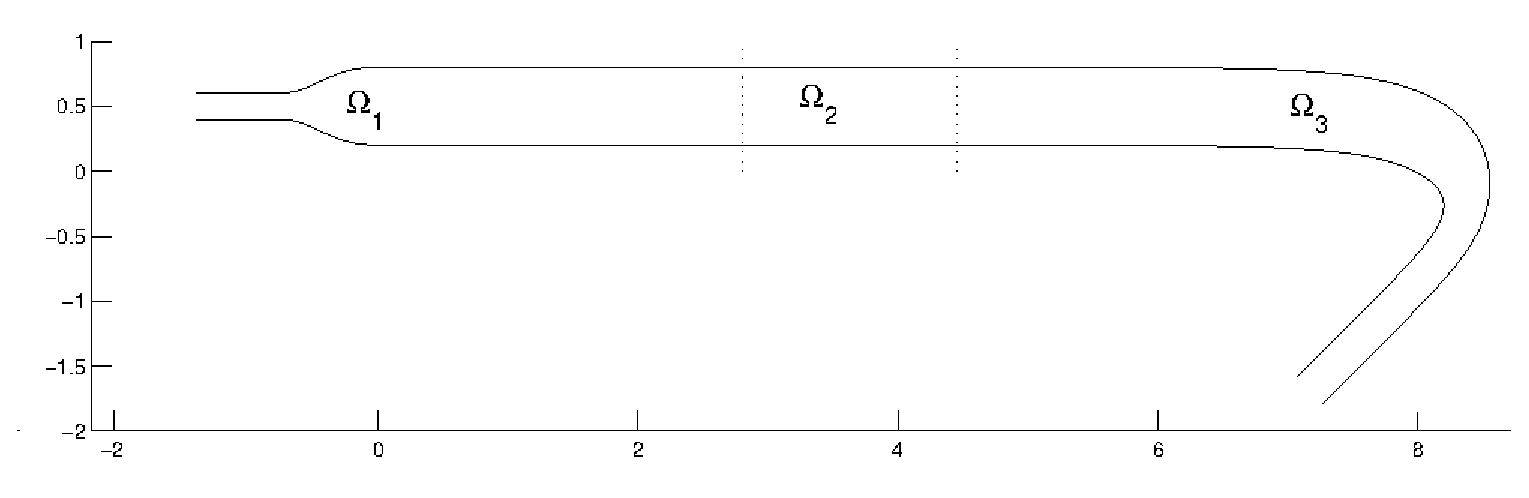
\includegraphics[width=\textwidth]{waveguide.2}
%   \caption{Waveguides with bounded connecting regions between
%   straight waveguide sections.}
%   \label{fig:wg2}
% \end{figure}
% Solutions $R^{A}$ and $T^{CA}$ to (\ref{108}) will be expressed in
% the solutions to two auxiliary problems that are easier to solve
% than (\ref{108}).  These auxiliary scattering problems must,
% however, be solved for incident waves from both left and right, the
% first being transition one between the straight waveguides $A$ and
% $B$ shown in Fig.~\ref{fig:wg2}b. For this transition%
% \begin{equation}
%   \left\{
%     \begin{array}
%       [c]{l}%
%       p=p_{+}^{A,\text{ in}}+R_{1}^{A}p_{+}^{A,\text{ in}}+T_{1}^{AB}p_{-}^{B,\text{
%           in}}\text{ in }A\\[1ex]
%       p=p_{-}^{B,\text{ in}}+R_{1}^{B}p_{-}^{B,\text{ in}}+T_{1}^{BA}p_{+}^{A,\text{
%           in}}\text{ in }B
%     \end{array}
%   \right.  \label{109}%
% \end{equation}
% defines the reflection operators $R_{1}^{A}$: $X_{+}^{A}\rightarrow
% X_{-}^{A}$ and $R_{1}^{B}$: $X_{-}^{B}\rightarrow X_{+}^{B}$
% together with the transmission operators $T_{1}^{BA}$:
% $X_{+}^{A}\rightarrow X_{+}^{B}$ and $T_{1}^{AB}$:
% $X_{-}^{B}\rightarrow X_{-}^{A}.$ Corresponding definitions for
% connecting region 2 between waveguides $B$ and $C,$ see
% Fig.~\ref{fig:wg2}c are%
% \begin{equation}
%   \left\{
%     \begin{array}
%       [c]{l}%
%       p=p_{+}^{B,\text{ in}}+R_{2}^{B}p_{+}^{B,\text{ in}}
%       +T_{2}^{BC}p_{-}^{C,\text{in}}\text{ in }B\\[1ex]
%       p=p_{-}^{C,\text{ in}}+R_{2}^{C}p_{-}^{C,\text{ in}}+
%       T_{2}^{CB}p_{+}^{B,\text{in}}\text{ in }C
%     \end{array}
%   \right.  ,\label{110}%
% \end{equation}
% where the domain and the range for the reflection and transmission
% operator are defined in analogy with those for (\ref{109}).

% By using linearity and (\ref{108}--\ref{110}) we get%
% \begin{equation}
%   \left\{
%     \begin{array}
%       [c]{l}%
%       R^{A}p_{+}^{A,\text{ in}}=R_{1}^{A}p_{+}^{A,\text{in}}
%       +T_{1}^{AB}p_{-}\\[1ex]
%       p_{+}=R_{1}^{B}p_{-}+T_{1}^{BA}p_{+}^{A,\text{ in}}\\[1ex]
%       p_{-}=R_{2}^{B}p_{+}\\[1ex]
%       T^{CA}p_{+}^{A,\text{ in}}=T_{2}^{CB}p_{+}%
%     \end{array}
%   \right.  \label{111}%
% \end{equation}
% for the waveguide with two connecting regions,
% Fig.~\ref{fig:wg2}a. The first equation in (\ref{111}) expresses
% that the minus or leftgoing wave in A consists of a sum of the
% reflected wave in the first connecting region plus the transmission
% from $B.$ Equations two and three describe the relations in $B$
% whereas the fourth equation gives the transmission to $C.$

% A combination of the second and third equation in (11) yields
% \begin{equation}\label{112}
%   (I_{+}^{B}-R_{1}^{B}R_{2}^{B})p_{+}=T_{1}^{BA}p_{+}^{A,\rm{in}},
% \end{equation}
% where $I_{+}^{B}$ is the unit operator on $X_{+}^{B}$. If we assume
% that the operator $T_{+}^{BA}:X_{+}^{B}\rightarrow X_{+}^{B}$ exists
% where
% \begin{equation}\label{113a}
%   T_{+}^{BA}=(I_{+}^{B}-R_{11}^{B}R_{2}^{B})^{-1}T_{1}^{BA},
% \end{equation}
% the final result
% \begin{equation}\label{BBfinal}
%   \left\{
%     \begin{array}
%       [c]{l}%
%       R^A=R_1^A+T_1^{AB}R_2^{B}T_+^{BA}\\
%       T^{CA}=T_2^{CB}T_+^{BA}\\
%       p=(R_2^{B}T_+^{BA}+T_+^{BA})^{-1}p_+^{A,\rm{in}}\, \rm{in}~ B\\
%     \end{array}
%   \right.
% \end{equation}
% is received.


% % A combination of the second and third equation in (\ref{111})
% % yields%
% % \begin{equation}
% %   \left( I_{+}^{B}-R_{1}^{B}R_{2}^{B}\right)
% %   p_{+}=T_{1}^{BA}p_{+}^{A,\text{in}}, \label{112}%
% % \end{equation}
% % where $I_{+}^{B}$ is the unit operator in $X_{+}^{B}.$ If we
% % assume
% % that $\left( I_{+}^{B}-R_{1}^{B}R_{2}^{B}\right) ^{-1}$:
% % $X_{+}^{B}\rightarrow X_{+}^{B},$ exists, the final result
% % \begin{equation}
% %   \left\{
% %     \begin{array}
% %       [c]{l}%
% %       R^{A}=R_{1}^{A}+T_{1}^{AB}R_{2}^{B}
% %       \left(I_{+}^{B}-R_{1}^{B}R_{2}^{B}\right)^{-1}T_{1}^{BA}\\
% %       T^{CA}=T_{2}^{CB}
% %       \left(I_{+}^{B}-R_{1}^{B}R_{2}^{B}\right)^{-1}T_{1}^{BA}%
% %     \end{array}
% %   \right.  , \label{113}%
% % \end{equation}
% % is received.

% Methods like (\ref{BBfinal}) have been known since the end of the
% 1940:s \cite{kerns1949} and are denoted the Building Block method
% \cite{nilssonbrander1981b} in acoustic theory and cascade technique
% \cite{jones1986} in electromagnetic theory.

% For a numerical solution, (\ref{BBfinal}) is transferred to a matrix
% equation by a truncated expansion in waveguide modes. Unless the
% wavelength is much smaller than the transverse dimension of the
% wavelength, the required size of the matrix representing
% $I_{+}^{B}-R_{1}^{B}R_{2}^{B}$ to get sufficient accuracy is
% small. The reason is that matrix elements, except for the lowest, is
% usually $O(ka),$ when $ka$ tends to zero where $a$ is a typical
% transverse dimension of the waveguide. This has been proved for
% specific geometries
% \cite{boijnilsson2003,boijnilsson2006,nilsson1998}. The Building
% Block Method, described above, assumes that there is a straight
% connecting waveguide between the two connecting regions. If this is
% not the case, such a straight part of length $\delta$ can be
% introduced and letting $\delta$ tend to zero at the end of the
% analysis. The convergence of this procedure is rather quick as
% demonstrated for a few cases \cite{nilssonbrander1981b}.

% This section is ended with a discussion of existence and uniqueness
% of the solutions to (\ref{108}-\ref{110}) and (\ref{BBfinal}),
% starting with the cases $\beta=0$ and $\beta=\i\infty$ for the
% connecting regions; in the straight parts $\beta$ is assumed to
% vanish. With our assumptions about the boundary of connecting
% region, the Fredholm alternative holds \cite{cessenat1996} for the
% scattering problems (\ref{108}-\ref{110}). More precisely, we have
% either (a) the homogeneous problem without incident waves has the
% unique solution $p=0;$ then the scattering problem is uniquely
% solvable or (b) the homogeneous problem has non-trivial solutions
% $p=p_{\text{hom}}$, which happens for $k$ belonging to a discrete
% set $\mathcal{K}=\left\{ k=k_{i}\text{:
% }k_{1}<k_{2}<k_{3}<\ldots\right\} ;$ then the solution
% $p=p_{\text{inhom}}+p_{\text{hom}}$ to the scattering problem exists
% but the homogeneous solution $p_{\text{hom}}$ is undetermined
% denoted a trapped mode. Consequently, the inverse $\left(
%   I_{+}^{B}-R_{1}^{B}R_{2}^{B}\right)^{-1}$ exists for all positive
% $k$ except for a countable set.

% The Fredholm alternative holds for case $\beta\neq0$ although it is
% not established in the cited reference \cite{cessenat1996} and no
% proof is presented here. A trapped mode cannot exist in a region
% where $\Re\beta>0$ due to energy conservation. Since a trapped mode
% cannot be compactly supported due to the analytic property of the
% solution to Helmholtz equation, we formulate the proposition that
% the scattering problem is uniquely solvable if there is a finite
% region with $\Re\beta>0.$

\section{Solving the one-block problems}
\label{sec:oneblock}

Wave scattering in a complicated geometry with varying boundary
conditions can be treated as a series of simpler problem, using the so
called Building Block Method, see
Section~\ref{sec:comb-blocks-build}. The method determines reflection
and transmission operators for the waveguide, given that these
operators have been determined for each section (``block'') of the
waveguide. 

In this section, we show how reflection and transmission operators for
a single block are established, but also, using a Dirichlet-to-Neumann
formulation, how the acoustic wave field inside the block could be
determined.  When performing these calculations, interactions from the
two ends of the block must be avoided, and hence, each block is
assumed to be an infinitely long waveguide with parallel straight
walls and constant boundary conditions outside some bounded transition
region.

In each such geometry, the boundary value problem
\begin{equation}
  \label{eq:bvp1}
  \begin{cases}
    \left(\nabla^2+k^2\right)p(x,y)=0&\text{in the waveguide,}\\[1ex]
    \pd pn=\i k\beta(t)p&\text{on the boundary,}
  \end{cases}
\end{equation}
where $\beta$ varies smoothly with some boundary parameter $t$, should
be solved. For the sake of simplicity, we assume that one of the
channel walls is hard, giving a Neumann boundary condition there.

We use a conformal mapping
\begin{equation*}
  F:w=u+\i v\to z=x+\i y
\end{equation*}
to transform the geometry into a straight horizontal channel
\mbox{$\{u\in\R,0\le v\le1\}$} in the $(u,v)$-plane, see
Fig.~\ref{fig:confmap}. After this transformation, Eq.~(\ref{eq:bvp1})
yields
\begin{equation}
  \label{eq:bvp2}
  \begin{cases}
    \left(\nabla^2+k^2\mu(u,v)\right)\Phi(u,v)=0\\[1ex]
    \left.\pd{\Phi(u,v)}v\right|_{v=1}=\i kY(u)\Phi(u,1)\\[1.5ex]
    \left.\pd{\Phi(u,v)}v\right|_{v=0}=0
  \end{cases}
\end{equation}
where $\mu(u,v)=\abs{F'(w)}^2$ and $Y(u)=\beta(u)\abs{F'(u+i)}$.
\begin{figure}[htb]
  \centering
  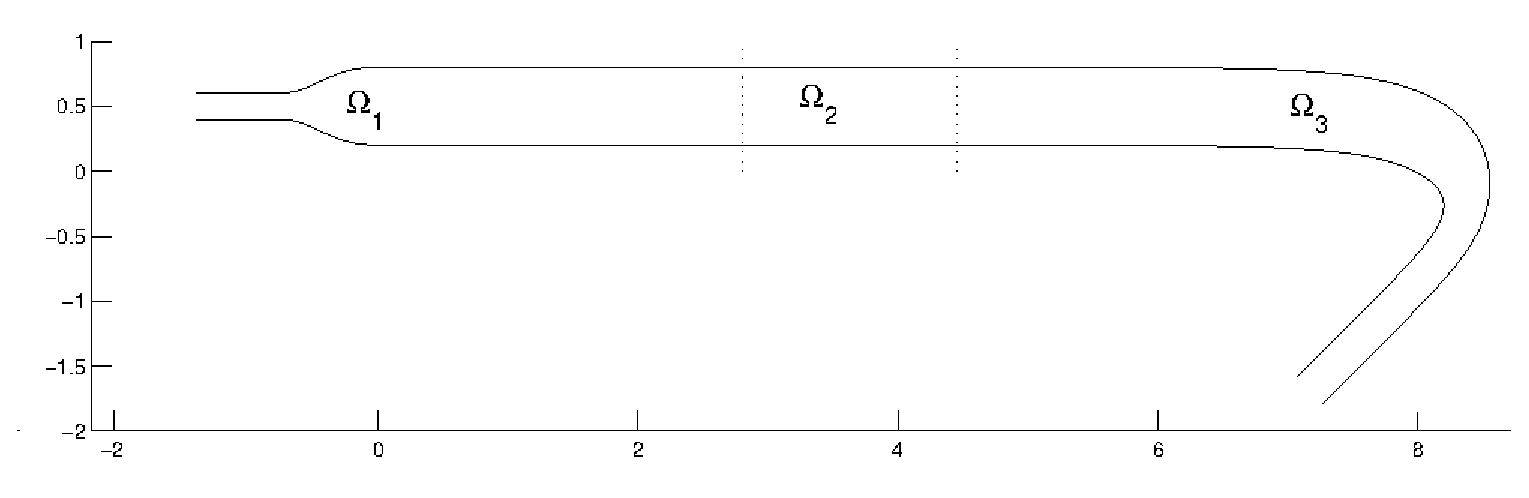
\includegraphics[scale=1]{waveguide.3}
  \caption{A single block in the $z=x+\i y$ plane and the $w=u+\i v$
    plane.}
  \label{fig:confmap}
\end{figure}

Following the techniques, outlined in \cite{Andersson-Nilsson:2009},
where an electro-magnetic scattering problem is treated, or
\cite{Nilsson:2002}, where similar problems from acoustics are solved,
we expand $\Phi(u,v)$ in cosine Fourier series over $v$, assuming that
\begin{equation}
  \label{eq:fcosseries}
  \Phi(u,v)=\sum_n\Phi_n(u)\phi_n(u,v),
\end{equation}
where $\phi_n(u,v)=\cos(v\lambda_n(u))$ for functions
$\lambda_n(u),\quad n\in\mathbb N$.

The functions $\lambda_n$ are determined by the boundary condition
(\ref{eq:bvp2}), from which follows that $\lambda_n(u)$,
$n=0,1,\dots$, are solutions to the equation
\begin{equation}
  \label{eq:lambdaeq}
  \lambda_n(u)\tan\bigl(\lambda_n(u)\bigr)=-\i kY(u).
\end{equation}
By differentiating (\ref{eq:lambdaeq}), it follows that
\begin{equation}
  \label{eq:lambdaprim}
  \lambda_n'(u)=
  \frac{-\i kY'(u)}{Q(u)}
\end{equation}
and
\begin{equation}
  \label{eq:lambdabis}
  \lambda_n''(u)=-\i k\left(\frac{Y''(u)Q(u)-Y'(u)Q'(u)}
    {\bigl(Q(u)\bigr)^2}\right)
\end{equation}
where $(')$ stands for differentiating with respect to $u$ and
\begin{equation*}
  Q(u)=\tan\bigl(\lambda(u)\bigr)+
  \lambda(u)\Bigl(1+\tan^2\bigl(\lambda(u)\bigr)\Bigr).
\end{equation*}

From the expansions
\begin{align}
  \label{eq:vsinlambda}
  &v\sin(v\lambda_n(u))=\sum_m\alpha_{mn}(u)\cos(v\lambda_m(u)),\\
  \label{eq:vcos^2lambda}
  &v^2\cos(v\lambda_n(u))=\sum_m\beta_{mn}(u)\cos(v\lambda_m(u)),\\
  \label{eq:mucoslambda}
  &\mu(u,v)\cos(v\lambda_n(u))=\sum_m\mu_{mn}(u)\cos(v\lambda_m(u)),
\end{align}
follows the infinite-dimensional ordinary differential equation
\begin{equation}
  \label{eq:DE}
  \vec\Phi''(u)-A(u)\vec\Phi'(u)-B^2(u)\vec\Phi(u)=0,
\end{equation}
where the infinite vector $\vec\Phi=(\Phi_1 \Phi_2 \Phi_3\dots)^T$ and
the infinite matrices $A$ and $B^2$ have elements
\begin{equation}
  \label{eq:A}
  A_{mn}(u)=2\alpha_{mn}(u)\lambda_n'(u)
\end{equation}
and
\begin{equation}
  \label{eq:B2}
  B^2_{mn}(u)=\alpha_{mn}(u)\lambda_n''(u)
  +\beta_{mn}(u)\left(\lambda_n'(u)\right)^2
  +\delta_{mn}\left(\lambda_n(u)\right)^2
  -k^2\mu_{mn}(u).
\end{equation}

Note that $(\varphi_m)$, with $\varphi_m(v)=\cos v\lambda_m(u)$, is in
general not an orthogonal system since the eigenvalue problem
(\ref{eq:bvp2}) is a regular Sturm-Liouville problem only if $Y$ is
purely imaginary. However, $(\varphi_m)$ and $(\overline{\varphi_m})$,
with a bar $\overline{\cdot}$ denoting the complex conjugate, form a
biorthogonal system meaning that the bilinear form
\begin{equation}\label{eq:bilinear}
  \langle \varphi_m,\varphi_n\rangle 
  =(\varphi_m,\overline{\varphi_n})
  =\int_0^1\varphi_m(v)\varphi_n(v){\rm d}v,
\end{equation}
vanishes if $n\neq m$. Here, for complex functions $f$ and $g$,
$(f,g)$ denotes the complex scalar product and the bilinear form
$\langle f,g \rangle$ is formally the same as the real scalar
product. This means that the expansion coefficients like
$\alpha_{mn}(u),\beta_{mn}(u)$ and $\mu_{mn}(u)$ in
(\ref{eq:vsinlambda}--\ref{eq:mucoslambda}), are found from
\begin{equation}\label{eq:am}
 a_m=\frac{\langle f,\varphi_m \rangle}{\langle \varphi_m,\varphi_m \rangle}
\end{equation}
for the expansion
\begin{equation}\label{eq:expansion}
  f=\sum_m a_m \varphi_m.
\end{equation}

Furthermore, the system $(\varphi_m)$ is proved to be complete in
$L^2(0,1)$ using Hilbert space techniques
\cite{Bauer:1964},\cite{Bauer:1965} but Paley-Wiener space techniques
\cite{Young:1981} could also be used; see also \cite{Locker:2000} for
a general treatise on eigenvalue problems based on functional analysis
for differential equations with two-point boundary conditions such
that like (\ref{eq:bvp2}), the related operator is
non-self-adjoint. It is also worth noting \cite{Glav:2000} that the
completeness property for $(\varphi_m)$ can be analysed as an analytic
continuation of (\ref{eq:am}) from purely imaginary $Y$, for which
completeness holds, to general $Y$.


\subsection{Conformal mapping techniques}
\label{sec:confmap}

There are two indispensable requirements on the conformal
mapping. When determining reflection and transmission operators for a
single waveguide block, as well as the field inside the block, we must
assume no interactions from the ends of the block. This is
accomplished by treating the block as an infinite waveguide which is
straight and has constant cross-sections outside some bounded
region. We must therefore numerically construct a conformal mapping
from a straight infinite channel to an infinite channel in which the
walls at both ends are (at least) asymptotically straight and
parallel. Furthermore, to avoid singularities in the operators $A$ and
$B^2$ in the differential equation (\ref{eq:DE}), it follows from
(\ref{eq:bvp2}) that the mapping must have a bounded first derivative
on the boundary, and additionally, from (\ref{eq:lambdaprim}),
(\ref{eq:lambdabis}), (\ref{eq:A}) and (\ref{eq:B2}), bounded second
and third derivatives if the boundary has non-zero admittance.

In \cite{andersson-outpol:2008} and \cite{andersson-acf:2009},
conformal mapping techniques, suitable for this situation, are
developed. Both methods are built on the \scm, which guarantees that
the resulting channel walls are asymptotically straight and parallel
towards infinity, and they both result in regions with smooth boundary
curves, meaning that no singularities are introduced by the
mapping. In \cite{andersson-outpol:2008}, a suitable polygon,
surrounding the region under consideration, is determined, and the
conformal mapping is constructed by using the \scm\ for that
polygon. In \cite{andersson-acf:2009}, the factors in a \scm\ are
replaced by so called approximate curve factors that round the corners
in a way that gives a smooth boundary curve.

\subsection{Accomplishing stable equations}
\label{sec:stableeq}
The differential equation~(\ref{eq:DE}) cannot be solved directly by
numerical methods. However, there exist reformulations of
(\ref{eq:DE}) that are numerically stable for all but a countable set
of $k$, i.e. for $k\notin\{k_1,k_2,k_3,\dots\}$. In this section, we
describe two such reformulations, built on two different partitions of
the wave field $\vec\Phi$.

Recall that the block is assumed to be an infinitely long waveguide
which is straight and has parallel hard boundaries outside some
central transition region. Let $\Omega_L$ and $\Omega_R$ be the
straight regions to the left and right respectively.  In $\Omega_L$
and $\Omega_R$, the operator $A$ is zero, while $B$ is
constant. Assume that $B=B_-$ in $\Omega_L$ and $B=B_+$ in
$\Omega_R$. In $\Omega_L$ and $\Omega_R$, $B^2$ is a real constant
diagonal matrix, and to be consistent with standard theory for
straight waveguides, the square roots of $B^2$ are chosen such that
$B_-$ and $B_+$ have either positive real or negative imaginary
diagonal elements.

\subsubsection{Determining Reflection and Transmission operators (The
  RT method)}
\label{sec:RT}

% With the Building Block Method, see
% Section~\ref{sec:comb-blocks-build}, reflection and transmission
% operators for a waveguide, splitted in several blocks, can be
% calculated. To be able to use the method, reflection and transmission
% operators for each single block must be determined. This can be done
% without any prior determination of the field inside the block, by a
% reformulation of (\ref{eq:DE}) into numerically stable differential
% equations in terms of $R^+$, $R^-$, $T^+$ and $T^-$.


Inspired by the partition $p=p_-+p_+$ in a straight waveguide
where the two terms can be seen as representing waves marching from
left to right and right to left respectively, we make the following
definition: Let for all $u\in\R$, the wave field 
\begin{equation}
  \label{eq:Phipart1}
  \vec\Phi(u)=(\Phi_1(u)\ \Phi_2(u)\ \dots)^T
  =\vec\Phi^+(u)+\vec\Phi^-(u), 
\end{equation}
where $\vec\Phi^+(u)$ and $\vec\Phi^-(u)$ represent waves marching to
the right and left respectively.

Let furthermore $C$ and $D$ be operators, depending on $u$, such that
\begin{equation}
  \label{eq:plusminustodiff}
    \dfrac{\partial\vec\Phi}{\partial u}(u)=
    -C(u)\vec\Phi^+(u)+D(u)\vec\Phi^-(u),
\end{equation}
for all $u\in\R$. $C$ and $D$ can be defined in many different ways,
but they must be differentiable with respect to $u$, and since
(\ref{eq:DE}) must hold in $\Omega_L$ and $\Omega_R$ where $A(u)=0$,
it follows that $C=D=B_-$ in $\Omega_L$ and $C=D=B_+$ in
$\Omega_R$. We have used the definition
\begin{equation}
  \label{eq:CD}
  C(u)=D(u)=B_-+f(u)(B_+-B_-),
\end{equation}
where $f$ is a smooth function that is $0$ in $\Omega_L$ and $1$ in
$\Omega_R$. 

Define reflection and transmission
operators $R^+$, $R^-$, $T^+$, $T^-$, such that for $u_1<u_2$,
\begin{equation}
  \label{eq:RT}
  \begin{pmatrix}
    \vec\Phi^+(u_2)\\
    \vec\Phi^-(u_1)
  \end{pmatrix}=
  \begin{pmatrix}
    T^+(u_2,u_1)&R^-(u_1,u_2)\\
    R^+(u_2,u_1)&T^-(u_1,u_2)
  \end{pmatrix}
  \begin{pmatrix}
    \vec\Phi^+(u_1)\\
    \vec\Phi^-(u_2)
  \end{pmatrix}.
\end{equation}
This means that $T^-$ and $R^-$ transmits respectively reflects the
left-going waves $\vec\Phi^-$, while $T^+$ and $R^+$ transmits
respectively reflects the right-going waves $\vec\Phi^+$.


From (\ref{eq:DE}), (\ref{eq:Phipart1}) and
(\ref{eq:plusminustodiff}), it is possible to derive, for details see
for example \cite{Nilsson:2002}, the equation
\begin{equation}
  \label{eq:diffphiplusminus}
  \pd{}u
  \begin{pmatrix}
    \vec\Phi^+\\\vec\Phi^-
  \end{pmatrix}
  =
  \begin{pmatrix}
    J&K\\
    L&M
  \end{pmatrix}
  \begin{pmatrix}
    \vec\Phi^+\\\vec\Phi^-
  \end{pmatrix},
\end{equation}
where
\begin{equation}
  \label{eq:alphabeta}
  \begin{split}
    &J=(C+D)^{-1}\left(-C'-B^2+(A-D)C\right),\\
    &K=(C+D)^{-1}\left(D'-B^2-(A-D)D\right),\\
    &L=(C+D)^{-1}\left(C'+B^2-(A+C)C\right),\\
    &M=(C+D)^{-1}\left(-D'+B^2+(A+C)D\right).
  \end{split}
\end{equation}
% For simplicity, we assume that $C=D=B_-+f(u)(B_+-B_-)$, where $f$ is
% a regular real function such that $f(u)=0$ to the left and $f(u)=1$
% to the right.

For the determination of $T^+$ and $R^+$, we consider (\ref{eq:RT})
assuming that there are no sources in $\Omega_R$. Let $u_2\in\Omega_R$
be constant and let $u=u_1$ vary. This means that $\vec\Phi^-(u_2)=0$,
and (\ref{eq:RT}) simplifies to
\begin{equation}
  \label{eq:RT2}
  \begin{cases}
    T^+(u_2,u)\vec\Phi^+(u)=\vec\Phi^+(u_2),\\
    R^+(u_2,u)\vec\Phi^+(u)=\vec\Phi^-(u).
  \end{cases}
\end{equation}
By differentiating (\ref{eq:RT2}) with respect to $u$, we get
\begin{equation}
  \label{eq:RTdiff1}
  \begin{cases}
    \pd{T^+}u(u_2,u)\vec\Phi^+(u)+T^+(u_2,u)\pd{\vec\Phi^+}u(u)=0,\\[1.5ex]
    \pd{R^+}u(u_2,u)\vec\Phi^+(u)+R^+(u_2,u)\pd{\vec\Phi^+}u(u)=
    \pd{\vec\Phi^-}u(u),
  \end{cases}
\end{equation}
and using (\ref{eq:diffphiplusminus}) and (\ref{eq:RT2}) once more,
the Ricatti equations
\begin{align}
  \label{eq:Ricatti1}
  \begin{split}
    \pd{R^+}u(u_2,u)&=-R^+(u_2,u)\bigl(J(u)+K(u)R^+(u_2,u)\bigr)\\
    &\qquad\qquad\qquad\qquad\qquad+L(u)+M(u)R^+(u_2,u)
  \end{split}\\
  \label{eq:Ricatti2}
  \pd{T^+}u(u_2,u)&=-T^+(u_2,u)\bigl(J(u)+K(u)R^+(u_2,u)\bigr)\\
  \intertext{follow. For $R^-$ and $T^-$, we proceed similarly
    assuming no sources in $\Omega_L$, and deduce the equations}
  \label{eq:Ricatti3}
  \begin{split}
    \pd{R^-}u(u,u_1)&=-R^-(u,u_1)\bigl(M(u)+L(u)R^-(u,u_1)\bigr)\\
    &\qquad\qquad\qquad\qquad\qquad+K(u)+J(u)R^-(u,u_1),
  \end{split}\\
  \label{eq:Ricatti4}
  \pd{T^-}u(u,u_1)&=-T^-(u,u_1)\bigl(M(u)+L(u)R^-(u,u_1)\bigr).
\end{align}
Using truncated matrices in place of $J$, $K$, $L$ and $M$, these
equations can be solved numerically with an ordinary differential
equation solver. (\ref{eq:Ricatti1}) and (\ref{eq:Ricatti2}) are
solved from right to left using $R^+(u_2,u_2)=0$ and $T^+(u_2,u_2)=I$
as initial values, while (\ref{eq:Ricatti3}) and (\ref{eq:Ricatti4})
are solved from left to right, using $R^-(u_1,u_1)=0$ and
$T^-(u_1,u_1)=I$ as initial values.


\subsubsection{Determining the field (The DtN method)}
\label{sec:DtN}

To determine the field inside a single block, we reformulate
(\ref{eq:DE}) using Dirichlet-to-Neumann operators, see also
\cite{Lu:1999} and \cite{Fishman:1998}. For this purpose,
we make a different partition of $\vec\Phi$. Let
\begin{equation}
  \label{eq:phiRphiL}
  \vec\Phi=\vec\Phi_R+\vec\Phi_L,
\end{equation}
where $\vec\Phi_R$ are waves with no sources to the right (in
$+\infty$) and $\vec\Phi_L$ are waves with no sources to the left (in
$-\infty$). Define Dirichlet to Neumann (DtN) operators $\Lambda_R$
and $\Lambda_L$ such that
\begin{align}
  \label{eq:DtNdef1}
  &\vec\Phi_R'(u)=-\Lambda_R(u)\vec\Phi_R(u),\\
  \label{eq:DtNdef2}
  &\vec\Phi_L'(u)=\Lambda_L(u)\vec\Phi_L(u).
\end{align}
$\Phi_R$ and $\Phi_L$ are both satisfying (\ref{eq:DE}), and by
differentiating (\ref{eq:DtNdef1}) and (\ref{eq:DtNdef2}), the
operator equations
\begin{align}
  \label{eq:DtNDE1}
  &\Lambda_R'(u)=\bigl(A(u)+\Lambda_R(u)\bigr)\Lambda_R(u)-B^2(u)\\
  \label{eq:DtNDE2}
  &\Lambda_L'(u)=\bigl(A(u)-\Lambda_L(u)\bigr)\Lambda_L(u)+B^2(u)
\end{align}
follow. Since $A=0$ in $\Omega_L$ and $\Omega_R$,
\begin{align}
  \label{eq:LRDE1}
  &\vec\Phi_R'(u)+B_-\vec\Phi_R(u)=0,\quad
  \vec\Phi_L'(u)-B_-\vec\Phi_L(u)=0,&&u\in\Omega_L,\\
  \label{eq:LRDE2}
  &\vec\Phi_R'(u)-B_+\vec\Phi_R(u)=0,\quad
  \vec\Phi_L'(u)+B_-\vec\Phi_L(u)=0,&&u\in\Omega_R,
\end{align}
which means that if truncated matrices are used in place of $A$ and
$B^2$, (\ref{eq:DtNDE1}) and (\ref{eq:DtNDE2}) can be solved
numerically from right and left respectively, using the initial values
$\Lambda_R(u_2)=B_+$ and $\Lambda_L(u_1)=B_-$, where $u_1\in\Omega_L$
and $u_2\in\Omega_R$.  Finally, (\ref{eq:DtNdef1}) and
(\ref{eq:DtNdef2}) are solved numerically from left and right
respectively.

It is worth noticing that the Riccati
equations~(\ref{eq:Ricatti1}-\ref{eq:Ricatti4}) as well as
(\ref{eq:DtNDE1}-\ref{eq:DtNDE2}) can for a countable set of $k$
contain singularities for certain values of $u$ and resist a numerical
solution, for details and examples see for example
\cite{Fishman:1998}. However, these singularities appears for
$k$ values in the DtN equations (\ref{eq:DtNDE1}-\ref{eq:DtNDE2}) for
which the RT equations~(\ref{eq:Ricatti1}-\ref{eq:Ricatti4}) have no
problem, so the different methods complete each other
well. Furthermore, there exist numerical methods by which Riccati
matrix equations are integrated across singularities, even when no
knowledge about existence or placements of these is at hand, see for
example \cite{Li-Kahan:2012}.

% Note also that the reflection and transmission operators can be
% determined from $\Lambda_R$ and $\Lambda_L$. For details, see
% \cite{Fishman:1998}.

% For the determination of the field in the straight transition region
% between two blocks, we use (\ref{112}) and the third equation in
% (\ref{111}). Assuming no sources from the right side of the block to
% the right, we get
% \begin{equation}
%   \label{eq:Mp}
%   \begin{cases}
%     p_{+}=\left(I-R_{1}^{B}R_{2}^{B}\right)^{-1}
%     T_{1}^{BA}p_{+}^{A,\text{in}},\\
%     p_-=R_2^Bp_+,
%   \end{cases}
% \end{equation}
% where $p_+^{A,\text{in}}$ is the right-going part of the field to the
% left of the left block, $R_1^B$ and $T_1^{BA}$ are reflection and
% transmission operators for the block to the left, and $R_2^B$ is a
% reflection operator for the block to the right.

\section{Combining the Blocks - the Building Block Method}
\label{sec:comb-blocks-build}

The Building Block Method (BBM), see \cite{nilssonbrander1981b},
allows the determination of reflection and transmission operators for
a combination of several sections (``blocks'') of the waveguide, for
which these operators are known.  
% The
% equations~(\ref{eq:DtNDE1}--\ref{eq:DtNDE2}) tend often to be more
% stiff than the equations~(\ref{eq:Ricatti1}--\ref{eq:Ricatti4}), and
% hence, a better accuracy could be achieved using BBM, if no explicit
% determination of the field inside the blocks is required.

\begin{figure}[htb]
  \centering
  \includegraphics[width=\textwidth]{BBMwg.1}
  \caption{Waveguide divided in blocks. $\Omega_2$ is straight and
    with constant cross-section.}
  \label{fig:wg4}
\end{figure}


Assume that two subsequent blocks $\Omega_1$ and $\Omega_3$, are
connected by a region $\Omega_2$ which is straight and with constant
cross-section, see figure~\ref{fig:wg4}. 
%For simplicity, we assume
%that $\Omega_2$ is parallel to the $x$-axis. 
Furthermore, assume that
reflection and transmission operators in matrix form for $\Omega_1$
and $\Omega_3$ are known. 

In contrast to many descriptions of the BBM, we choose here to define
$\vec\Phi=\vec\Phi^++\vec\Phi^-$ as varying with the position along
the waveguide, even outside and between the blocks. The reflection and
transmission operators are defined accordingly: Assume that a block
begins and ends at position $a$ and $b$ respectively and that
there are no sources at the $b$ side of the block. If $T^+(=T^+(b,a))$
is the transmission operator for waves $\vec\Phi^+$ entering the block
at $a$, then $\vec\Phi^+(b)=T^+\vec\Phi^+(a)$ are the waves leaving
the block at position $b$. Let $t$ be a parameter, measuring the
distance along the central curve of the waveguide, and let $t=t_0$ at
the beginning (left end) of $\Omega_1$, $t=t_1=0$ at the border between
$\Omega_1$ and $\Omega_2$, $t=t_2=\ell$ at the border between $\Omega_2$
and $\Omega_3$, assuming that the length of $\Omega_2$ is $\ell$, 
 and finally $t=t_3$ at the end of
$\Omega_3$. Following the definitions given in Eq.~(\ref{eq:RT}), we
use the notation
\begin{align*}
  &R^+_1=R^+(t_1,t_0),&&T^+_1=T^+(t_1,t_0),\\
  &R^-_1=R^-(t_0,t_1),&&T^-_1=T^-(t_0,t_1),\\
  &R^+_3=R^+(t_3,t_2),&&T^+_3=T^+(t_3,t_2),\\
  &\Rtot=R^+(t_3,t_0),&&\Ttot=T^+(t_3,t_0).
\end{align*}
% \begin{center}
%   \begin{tabular}{ll}
%     Symbol&Explanation\\
%     \hline
%     {}\\[-2ex]
%     $R^{+}_1=R^+(t_1,t_0)$&Reflection operator for $\Omega_1$ for waves entering
%     from the left.\\
%     $T^{+}_1$&Transmission operator for $\Omega_1$ for waves entering
%     from the left.\\
%     $R^{-}_1$&Reflection operator for $\Omega_1$ for waves entering
%     from the right.\\
%     $T^{-}_1$&Transmission operator for $\Omega_1$ for waves entering
%     from the right.\\
%     $R^{+}_3$&Reflection operator for $\Omega_3$ for waves entering
%     from the left.\\
%     $T^{+}_3$&Transmission operator for $\Omega_3$ for waves entering
%     from the left.\\
%     $\Rtot$&Reflection operator for 
%     $\cup_{j=1}^3\Omega_j$ for waves entering
%     from the left.\\
%     $\Ttot$&Transmission operator for $\cup_{j=1}^3\Omega_j$ for
%     waves entering from the left.\\
%     \hline
%   \end{tabular}  
% \end{center}

For the straight part $\Omega_2$ with length $\ell$ and width $a$,
we define
\begin{equation}
  \label{eq:S}
  S(t)=
  \begin{pmatrix}
    \e^{\i\alpha_0t}&0&0&\cdots\\
    0&\e^{\i\alpha_1t}&0&\cdots\\
    0&0&\e^{\i\alpha_2t}&\\
    \vdots&\vdots&&\ddots
  \end{pmatrix},\quad 0\le t\le\ell,
\end{equation}
where $\alpha_n=\sqrt{k^2-\dfrac{n^2\pi^2}{a^2}}$.% and $x$ is the
%horizontal distance from the border between $\Omega_1$ and $\Omega_2$.

Assume that a right-marching field $\Phiin=\vec\Phi^+(t_0)$ is entering 
$\Omega_1$ from the left, and that there are no sources to the right of
$\Omega_3$. Define operators $C^\pm$ such that at the border between
$\Omega_1$ and $\Omega_2$, $\vec\Phi^+(0)=C^+\Phiin$ and
$\vec\Phi^-(0)=C^-\Phiin$. Standard theory for
straight waveguides gives that in $\Omega_2$ at position $t$, the
field is
\begin{equation}
  \label{eq:midfield}
  \vec\Phi(t)=(S(t)C^++S^{-1}(t)C^-)\Phiin.
\end{equation}
Consequently, at the border between $\Omega_2$ and $\Omega_3$, there
are right-marching and left-marching waves $S(\ell)C^+\Phiin$ and
$S^{-1}(\ell)C^-\Phiin$ respectively.

Since there are no sources to the right of $\Omega_3$,
$S^{-1}(\ell)C^-=R_3^{+}S(\ell)C^+$, so
$C^-=S(\ell)R_3^{+}S(\ell)C^+$. But $C^+=T_1^{+}+R_1^{-}C^-$, and
hence
\begin{equation}
  \label{eq:ABRtotTtot}
  \begin{split}
    &C^+=\left(I-R_1^{-}S(\ell)R_3^{+}S(\ell)\right)^{-1}T_1^{+},\\
    &C^-=S(\ell)R_3^{+}S(\ell)C^+,\\
    &\Ttot=T_3^{+}S(\ell)C^+,\\
    &\Rtot=R_1^{+}+T_1^{-}C^-.
  \end{split}
\end{equation}

The methods has been known since the end of the 1940:s
\cite{kerns1949} and is denoted the Building Block Method
\cite{nilssonbrander1981b} in acoustic theory and cascade technique
\cite{jones1986} in electromagnetic theory.



\section{A numerical example}
\label{sec:numerical-example}
To illustrate the techniques, we solve the scattering problem and
determine a low-frequency field in the waveguide shown in
Fig.~\ref{fig:exwg}.
\begin{figure}[htb]
  \centering \ifpdf
  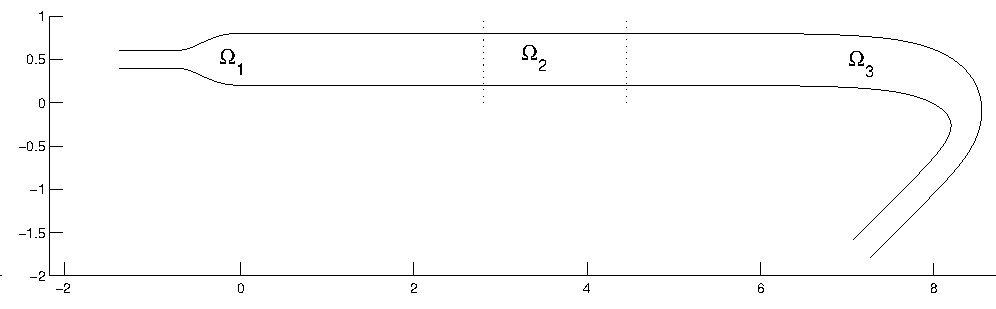
\includegraphics[width=\textwidth]{waveguide.jpg}
  \else
  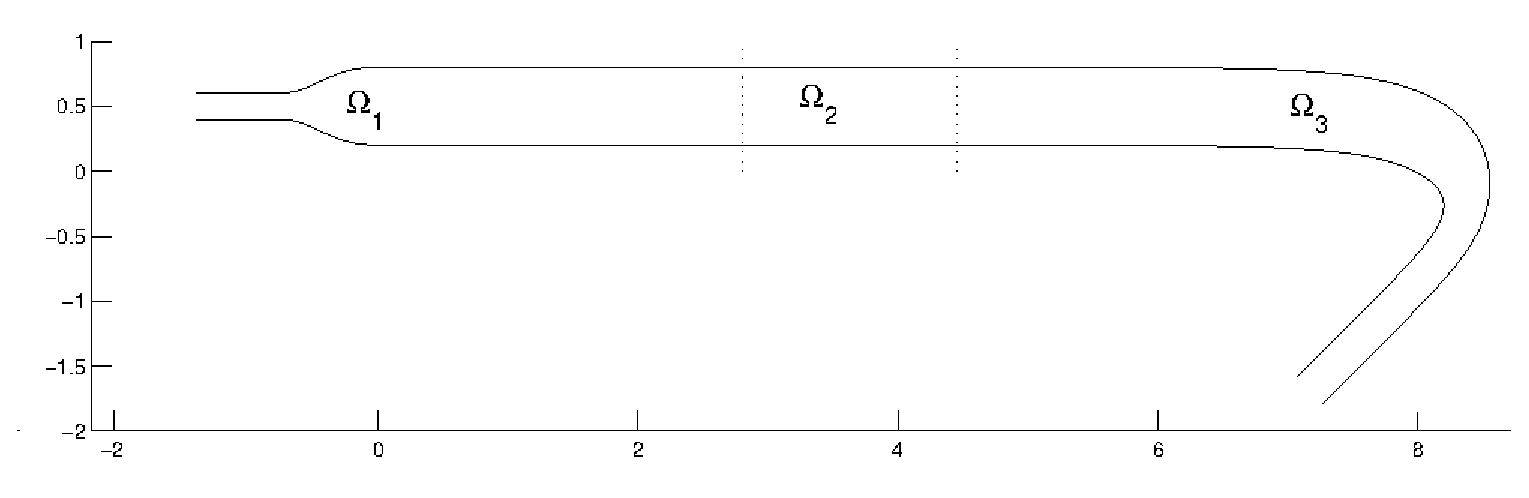
\includegraphics[width=\textwidth]{waveguide.eps}
  \fi
  \caption{The waveguide in the example.}
  \label{fig:exwg}
\end{figure}
The results, i.e., the acoustic field in the waveguide given a known
field entering from the left, as well as reflection as transmission
operators for the waveguide, are calculated and compared with a finite
element method solution.

\subsection{Boundary conditions}
\label{sec:boundary-conditions}

% In this geometry, we assume a smoothly and monotonuosly increasing
% admittance in the intervals $F_j([-2,-1]+\i)$, a constant admittance
% $\beta=0.5+0.5i$ in the intervals $F_j([-1,1]+\i)$, and finally
% smoothly monotonously decreasing admittance in the intervals
% $F_j([1,2]+\i)$, where the functions $F_j, j=1,2$ are the conformal
% mappings defined in Section~\ref{sec:conformal-mappings}. The
% remaining boundaries are hard.


The boundaries are hard, i.e., have zero admittance, except for two
intervals on the upper boundary. In both $\Omega_1$ and $\Omega_3$,
there is admittance at the upper boundary in the intervals
$F_j([-2,2]+\i)$ for $j\in\{1,2\}$, reaching the maximal level
$\beta=0.5+0.5\i$ in the intervals $F_j([-1,1]+\i)$, where the
functions $F_j$ are the conformal mappings defined in
Section~\ref{sec:conformal-mappings}. 
% Additionally, results for
% $\beta=0$ on all the boundary have also been calculated.

\subsection{Conformal mappings}
\label{sec:conformal-mappings}

The region is divided into three disjoint parts. $\Omega_1$ contains
the change in cross-section to the left, the middle section $\Omega_2$
is straight with constant cross-section, and $\Omega_3$ contains the
bending to the right.

For $\Omega_1$, shown in Fig.~\ref{fig:sc}(a), a conformal mapping is
constructed using the approximate curve factor technique developed in
\cite{andersson-acf:2009}. The conformal mapping is $F_1=f_1\circ
g_1$, where
\begin{equation}
  \label{eq:scconfmap1}
  f_1(w)=A\int_{w_0}^w
  \prod_{j=1}^4\left(
    \sqrt{(\omega+b_k\i-w_k)^2-c_k^2}-b_k\i
  \right)^{\alpha_k-1}\omega^{-1}d\omega+z_0,
\end{equation}
and
\begin{equation}
  \label{eq:scconfmap2}
  g_1(w)=\exp(\pi w).
\end{equation}
In (\ref{eq:scconfmap1}), $A=0.6/\pi$ to get the width $0.6$ to the
right, $\vec\alpha=(0.85,1.15,1.15,0.85)^t$ to get inner angles of
sizes $1.15\pi$ and $0.85\pi$, $\vec b=\vec c=(1,0.05,0.05,1)^t$ to
get the corners appropriately rounded, and $\vec w=(-1,-a,a,1)^t$,
where $a=0.008740$ has been numerically determined to get the width
$0.2$ to the left. Finally, $w_0$ is set to $2$ and $z_0$ to $1+0.2i$
to position the waveguide in the complex plane.
\begin{figure}[htb]
  \centering
  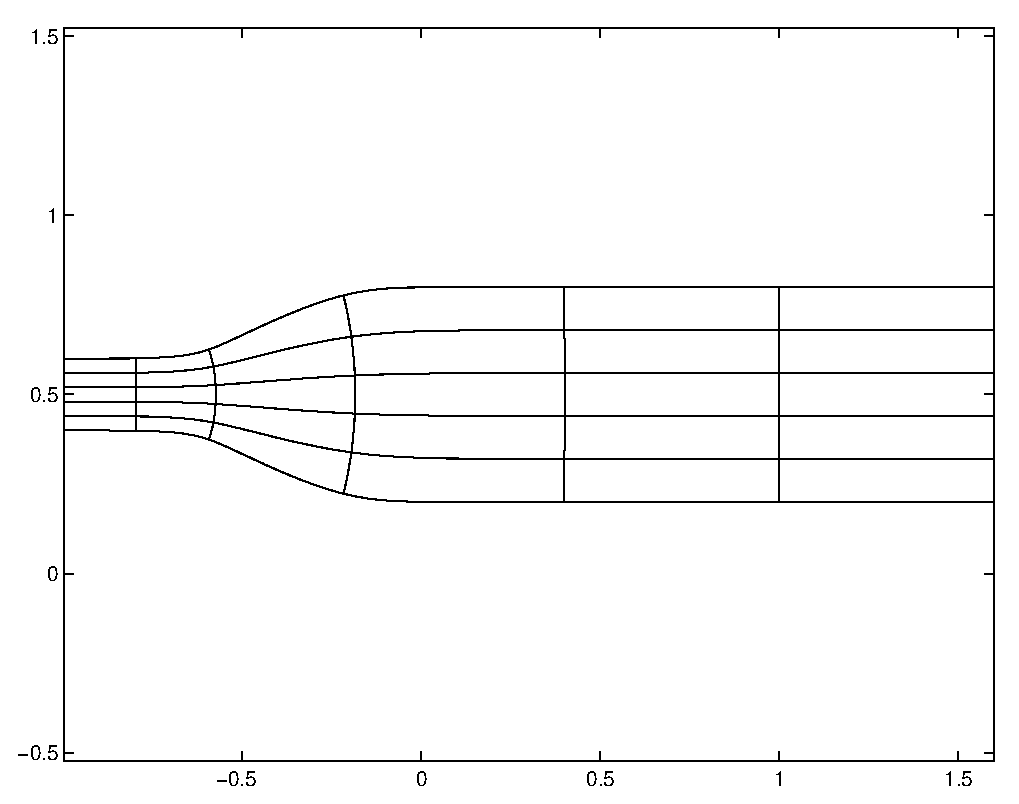
\includegraphics[width=0.45\textwidth]{sc}
  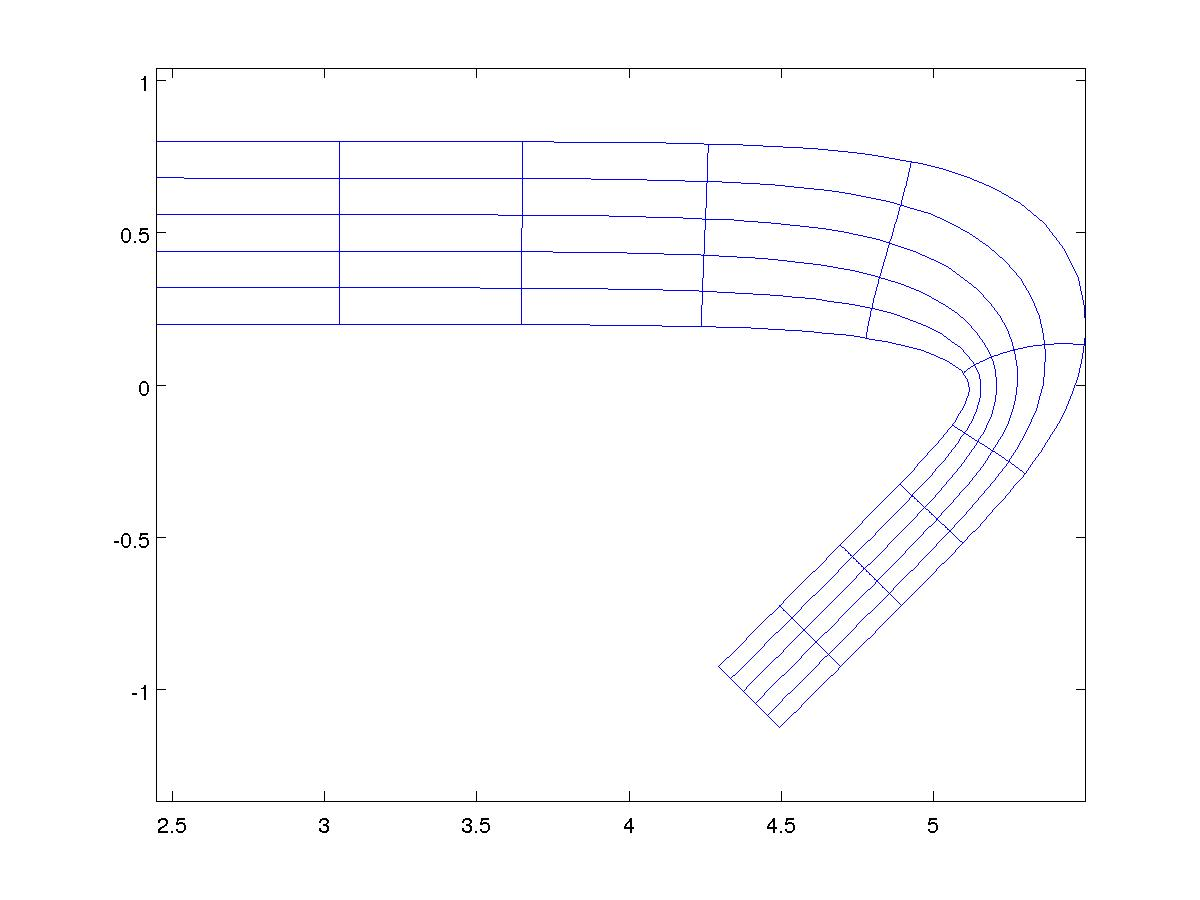
\includegraphics[width=0.45\textwidth]{bc}
  \caption{The two building blocks. The grid lines are images under the
    conformal mappings of $u=-5,-4,...,4,5$ and $v=0,0.2,\dots,1$.}
  \label{fig:sc}
\end{figure}

For $\Omega_3$, shown in Fig.~\ref{fig:sc}(b), the outer polygon
method \cite{andersson-outpol:2008} is used to construct the conformal
mapping. The mapping function is here $F_2=f_2\circ g_2$, where
\begin{equation}
  \label{eq:bcconfmap1}
  f_2(w)=\int_{g_2(w_0)}^w\frac{(\omega-1)^{\alpha-1}}
  {(\omega+1)^{\alpha-1}(\omega-a)}\,d\omega+z_0
\end{equation}
and
\begin{equation}
  \label{eq:bcconfmap2}
  g_2(w)=w^{(\phi_2-\phi_1)/\pi}\e^{\i\phi_1}+a,
\end{equation}
with $A=0.1501\exp(3\pi\i/4)$, $\alpha=7/4$, $\phi_1=3\pi/10$,
$\phi_2=7\pi/10$, $a=-0.4632$, $w_0=-7$ and $z_0=4.4485+0.2\i$.

\subsection{Determination of the field, reflection and transmission
  operators}
\label{sec:determ-field-refl}

The acoustic fields inside $\Omega_1$ and $\Omega_3$ have been
determined using the techniques described in
Section~\ref{sec:DtN}. Simultaneously, reflection and transmission
operators for $\Omega_1$ and $\Omega_3$ have been determined using the
techniques in Section~\ref{sec:RT}. All calculations have been made
using $10\times10$ matrices in place of the operators in the
differential equations (\ref{eq:Ricatti1})--(\ref{eq:Ricatti4}) and
(\ref{eq:DtNdef1}--\ref{eq:DtNDE2}) and a standard numerical ODE
solver (\verb+ode45+).

We have assumed a source at infinity to the left resulting in a
right-marching wave $\vec\Phi_{\text{in}}=(1\ 0\ 0\ 0\dots)^t$
entering the waveguide from the left. No sources to the right is
assumed.

The matrices $A(u)$ and $B^2(u)$ in (\ref{eq:DE}), as well as the
matrices $J$, $K$, $L$ and $M$ in (\ref{eq:alphabeta}) have been
determined for $u=-5,-4.99,...,5$ in $\Omega_1$, and for
$u=-7,-6.99,...,7$ in $\Omega_3$. Linear interpolation was then used
in the ODE solvers to determine $J$, $K$, $L$ and $M$ in
eqs. ~(\ref{eq:Ricatti1}--\ref{eq:Ricatti4}) and $A$ and $B^2$ in
eqs.~(\ref{eq:DtNDE1}) and (\ref{eq:DtNDE2}) for $u$ values not in
this set.

Finally, the field in $\Omega_2$ as well as reflection and
transmission operators for the whole waveguide was calculated using
the Building Block Method described in
Section~\ref{sec:comb-blocks-build}.

\subsection{Results}
\label{sec:results}

\begin{figure}[htb]
  \centering
  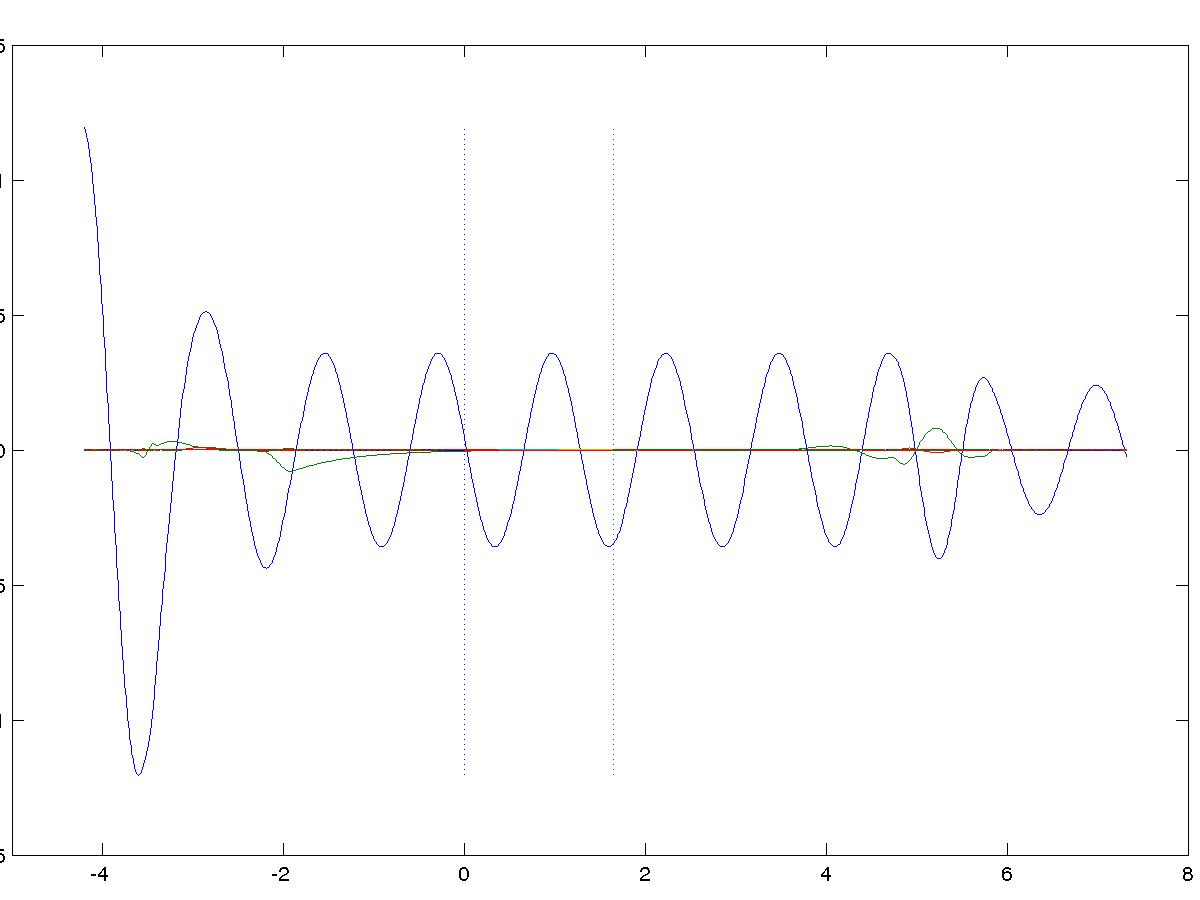
\includegraphics[keepaspectratio=false,width=\linewidth,
  height=3cm]{phin1a}
  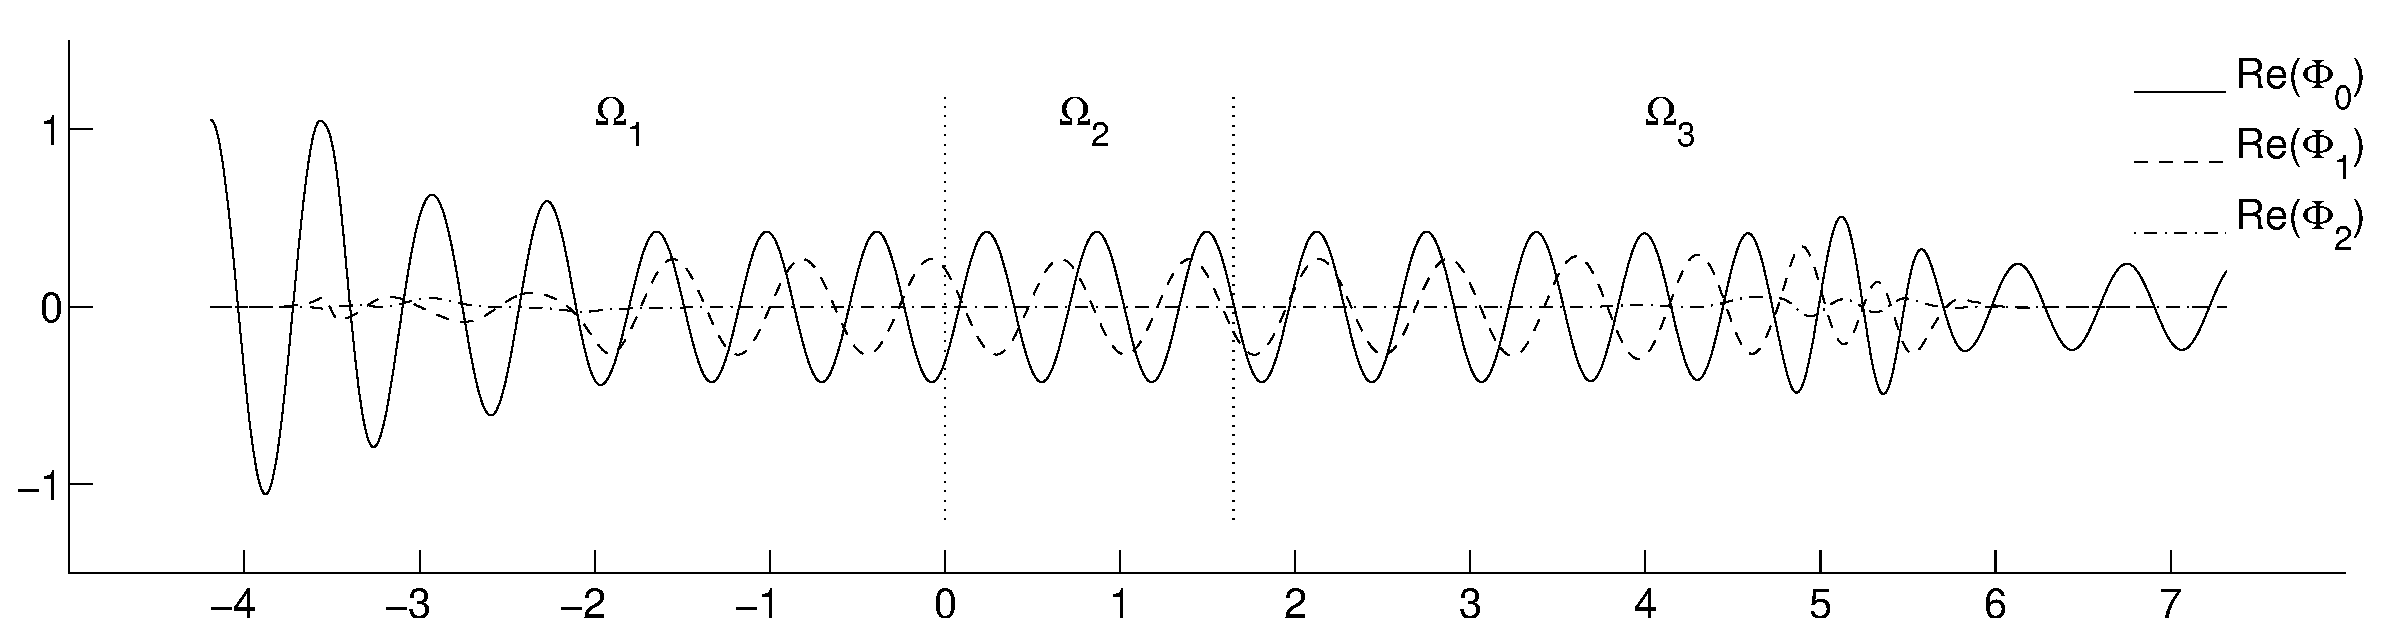
\includegraphics[keepaspectratio=false,width=\linewidth,
  height=3cm]{phin2a}
  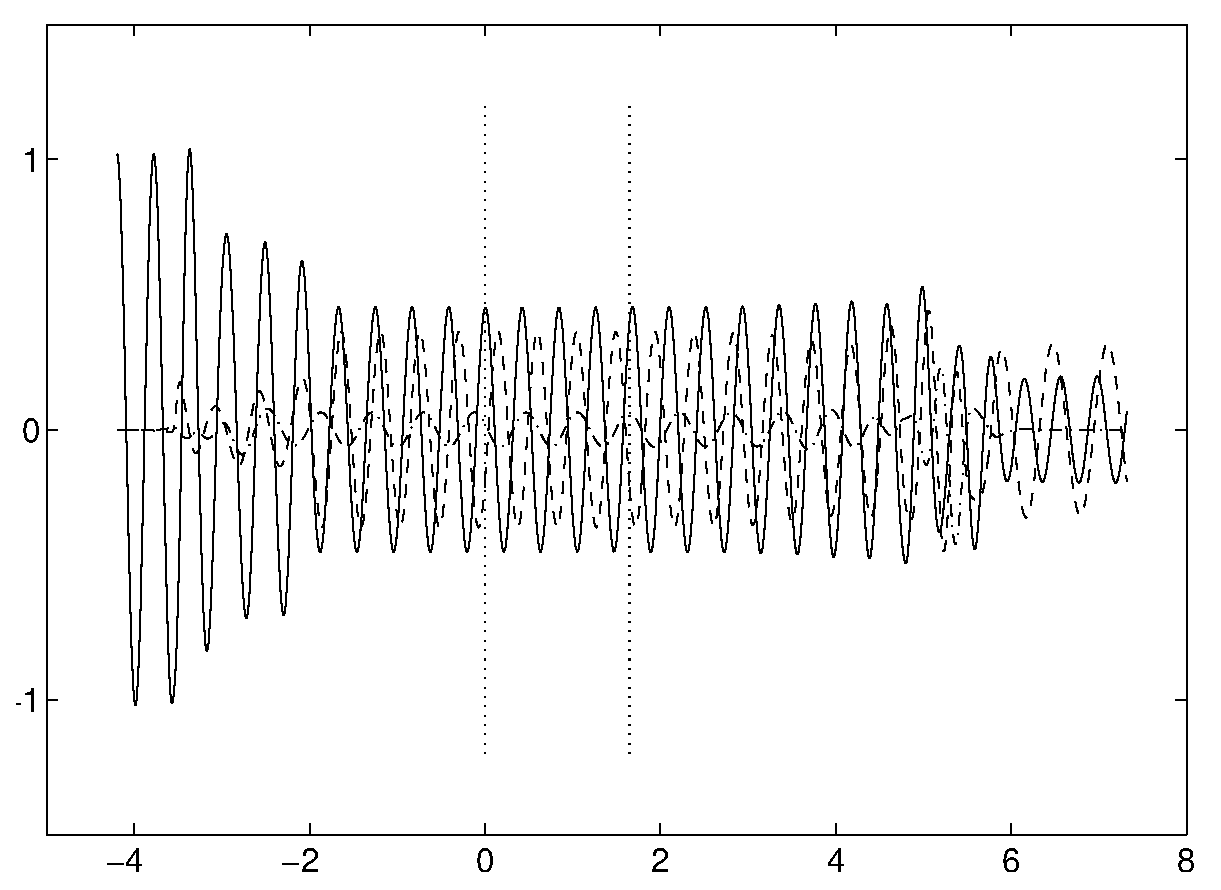
\includegraphics[keepaspectratio=false,width=\linewidth,
  height=3cm]{phin3a}
  \caption{$\Re\Phi_1,\Re\Phi_2,\Re\Phi_3,\dots$ for $k=5$, $k=10$ and
    $k=15$. Dotted vertical lines indicate borders between
    $\Omega_1$, $\Omega_2$ and $\Omega_3$.}
  \label{fig:phi}
\end{figure}

In Figure~\ref{fig:phi}, $\Re{\Phi_1},\Re{\Phi_2},\dots$ is plotted
for $k=5$, $k=10$ and $k=15$. The measure on the horizontal axis in
the plot is the distance along the central curve in the waveguide. In
Figure~\ref{fig:phitot3a}, a contour plot of $\Re p(x,y)$ is shown for
$k=15$.

\begin{figure}[ht]
  \centering
  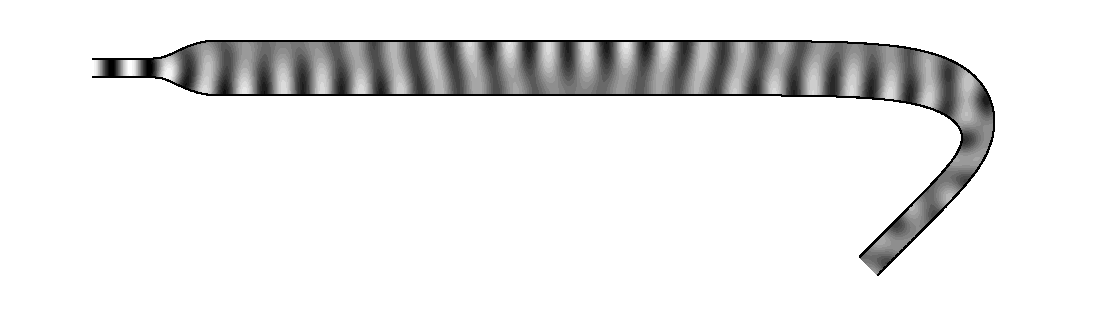
\includegraphics[width=\linewidth]{phitot3a}
  \caption{$\Re p(x,y)$ plotted for $k=15$.}
  \label{fig:phitot3a}
\end{figure}

\begin{table}[hb]
  \begin{equation*}
    \begin{array}{|l|rrl|}
      \hline
      &\multicolumn1c{\vec\Phi_{\Omega_1}(\text{end})}
      &\multicolumn1c{\vec\Phi_{\Omega_2}(0)}
      &\abs{\text{difference}}\\
      \hline
      \Phi_1&0.4521-0.0448\i&0.4521-0.0449\i&3.744\cdot10^{-5}\\
      \Phi_2&-0.1873-0.2693\i&-0.1873-0.2693\i&7.971\cdot10^{-6}\\
      \Phi_3&0.0190+0.0203\i&0.0190+0.0203\i&7.730\cdot10^{-6}\\
      \hline 
      &\multicolumn1c{\vec\Phi_{\Omega_3}(\text{end})}
      &\multicolumn1c{\Ttot\Phiin}
      &\\
      \hline
      \Phi_1&0.0671-0.1847\i&0.0671-0.1848\i&2.792\cdot10^{-5}\\
      \Phi_2&-0.1926+0.2528\i&-0.1926+0.2528\i&2.812\cdot10^{-5}\\
      \hline
    \end{array}
  \end{equation*}
  \caption{Comparing the RT and DtN method. Above: $\Phi_1$, $\Phi_2$
    and $\Phi_3$ at the border between $\Omega_1$ and $\Omega_2$
    calculated with the two different methods. Below:
    $\Phi_1$ and $\Phi_2$ at the end of $\Omega_3$
    calculated with the two different methods. All calculations are
    made for  $k=15$.}
  \label{tab:phires-bcend}
\end{table}

Note that in $\Omega_1$, $\vec\Phi$ is calculated using the methods in
Section~\ref{sec:DtN}, while in $\Omega_2$, where it is calculated
using (\ref{eq:midfield}) and (\ref{eq:ABRtotTtot}), $\vec\Phi$
depends on the reflection and transmission operators found by the
methods in Section~\ref{sec:RT}. It is therefore interesting to
compare $\vec\Phi$ in the right end of $\Omega_1$ with $\vec\Phi$ in
the left end of $\Omega_2$, i.e. with $(C^++C^-)\Phiin$. Likewise, it
is interesting to compare $\vec\Phi$ at the end of $\Omega_3$,
calculated with the DtN method, with $\Ttot\Phiin$, where $\Ttot$ is
determined using the RT method and the Building block method. 

These comparisons are given in Table \ref{tab:phires-bcend}, and show
that the correspondence between the methods is good.

\subsection{A FEM solution to the problem}
\label{sec:fem-solution-problem}

\begin{figure}[htb]
  \centering
  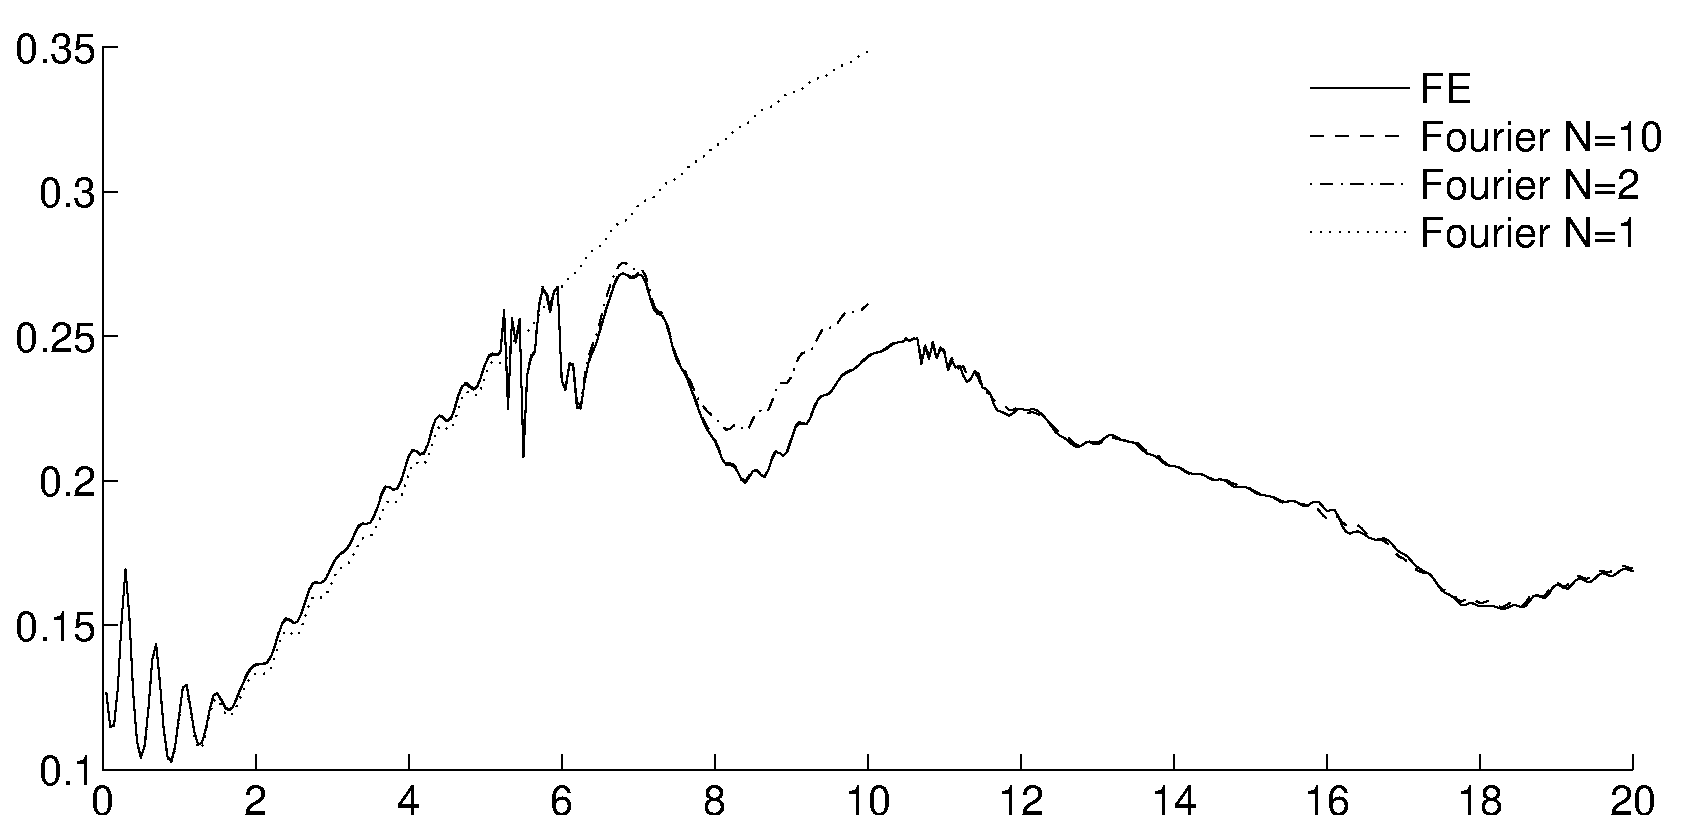
\includegraphics[keepaspectratio=false,height=5cm,width=\textwidth]
  {FEMvsFourier}
  \caption{$\abs{\Phi_{0}}$ at the end of $\Omega_3$ calculated for
    $k=0.05,0.1,\dots,20$ with the Fourier methods described in the
    article and with the Finite Element Method.}
  \label{fig:FEMvsFourier}
\end{figure}

The Finite Element Method (FEM) is a well-established process for
treating problems like the one in the example, and it is probably the
most used method to solve such problems. As a comparison, we have
applied a commercial FEM solver (COMSOL Multiphysics) to the
problem. In Figure~\ref{fig:FEMvsFourier}, FEM solutions for $k=0..20$
are compared with the corresponding Fourier method solutions. As is
seen in the figure, the correspondence is good. The differences
between the methods in the calculated $k$ interval are all less than
$4\cdot10^{-3}$.


\section{Discussion and conclusion}
\label{sec:conclusion}

% The technique used in the example can be extended to cover ... In
% the example, we have a smooth boundary and smoothly varying boundary
% conditions. A discontinuity in the geometry or in the boundary
% conditions can be treated by splitting the waveguide at the
% discontinuity in two new building blocks, and using for example mode
% matching techniques when gluing them together.

The example problem in Section~\ref{sec:numerical-example} is of
course not a ``general'' waveguide. There are numerous possible
boundary variations not commented so far. For example, the methods in
this article seem to require smooth changes in both geometry and
boundary conditions to get converging Fourier series. However, the
Building Block method and well-established mode-matching techniques
can overcome most such problems. Furthermore, as is illustrated in
\cite{Nilsson:2002} where an L-bend is investigated, good results can
be achieved even when the conformal mapping functions contain
singularities on the boundary. It is however evident that the
differential equations get stiffer and that larger truncated matrices
are required.

Another simplification in this article is the assumption of a Neumann
boundary condition on one of the boundaries. An iterated use of the
Building Block method and lengthways partitions of the waveguide can
handle two-dimensional waveguides with non-hard walls on both sides.

Finally, it is possible to extend the techniques to cover
three-dimensional problems, at least when variations in the geometry
take place in at most two dimensions at the time. We refer to the
discussion in \cite{Nilsson:2002}.

% Below follows a list of some
% such problems and suggestions how to treat them:

% \begin{description}
% \item[The boundary has sharp vertices.] When solving the one-block
%   problems with the methods described in Section~\ref{sec:oneblock},
%   we assume that the waveguide has smooth boundaries. Elsewise, the
%   $\mu$ function in (\ref{eq:bvp2}) will have singularities on the
%   boundaries. However, as is illustrated in... 
% \item[Sudden changes in the boundary conditions.] A disadvantage with
%   the Fourier methods seems to be that they require a boundary and
%   boundary conditions with a high degree of smoothness. In the example
%   in Section~\ref{sec:numerical-example}, this is the case. If not,
%   the first and second derivatives of the $\lambda$ functions, used in
%   eqs.~(\ref{eq:A}) and (\ref{eq:B2}), will contain singularities.
%   However...
% \item[Varying boundary conditions in both boundaries.] In
%   Section~\ref{sec:oneblock}, we assumed that one of the boundaries
%   was hard. This made it possible to develop the field in the
%   waveguide in Fourier cosine series. If that is not the case...
% \item[Combinations of several different changes.]
% \item[Three-dimensional waveguides.] The methods are under certain
%   conditions applicable even in three-dimensional problems. If the
%   changes in geometry take place in at most two dimensions at the
%   time,...
% \end{description}

The most time-consuming part of the calculations is the determination
of the matrices $A$ and $B^2$ in (\ref{eq:DE}) for a large set of
$u$-values. For every value of $u$, $\lambda_n(u)$ for $n=0,\dots,N-1$
should be found by solving equation (\ref{eq:lambdaeq}) numerically.
The values of $\alpha$ and $\beta$ in eqs.~(\ref{eq:vsinlambda}) and
(\ref{eq:vcos^2lambda}) can be determined analytically, but for every
$u$, $N^2$ numerical integrations are needed to determine the values
of $\mu_{mn}(u)$ in Eq.~(\ref{eq:mucoslambda}). For values of $u$,
corresponding to hard boundaries, $\lambda_n=n\pi$ and the $\mu$
coefficients can be calculated using Fast Fourier Transforms, but for
values of $u$ corresponding to boundaries with admittance, a
comparatively slow numerical integration must be used for each matrix
element.

\begin{figure}[htb]
  \centering
  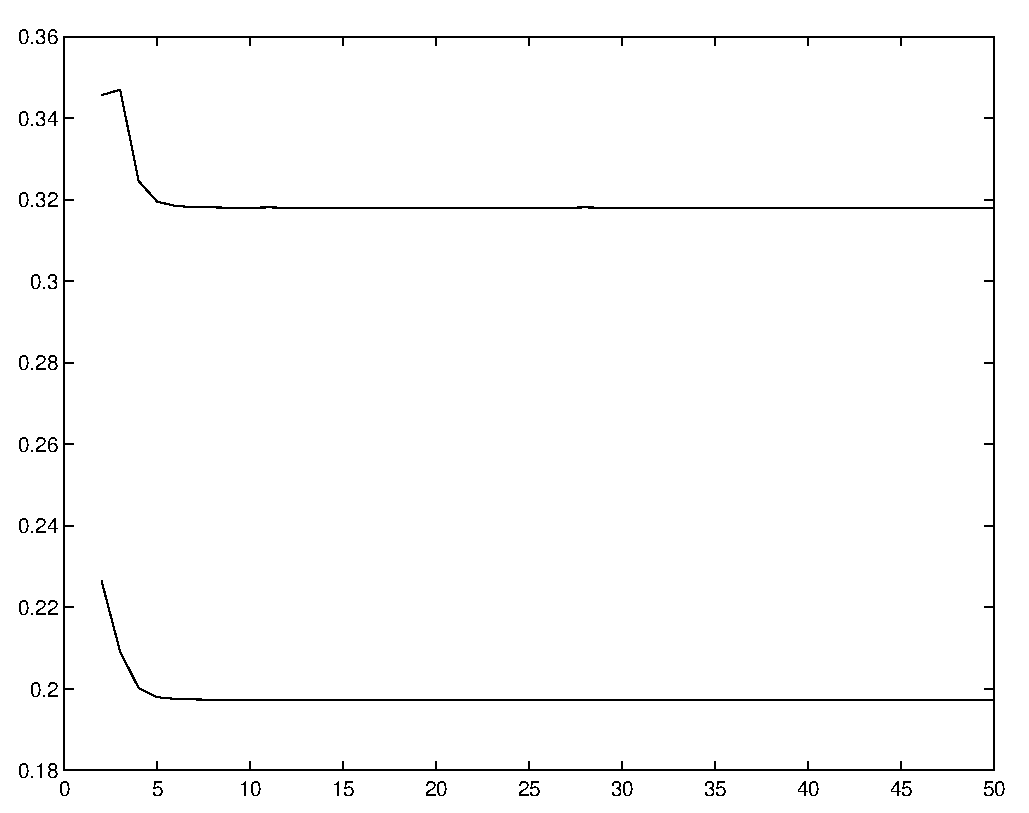
\includegraphics[keepaspectratio=false,width=0.7\linewidth,height=5cm]{T_N}
  \caption{$\abs{T^{\text{tot}}(0,0)}$ and $\abs{T^{\text{tot}}(1,0)}$
    for $k=15$ calculated using matrices of size $N\times N$ with
    $N=2\dots50$.}
  \label{fig:T_N}
\end{figure}

However, as is seen in Figure~\ref{fig:T_N}, for $k$ in the low
frequency domain that we have investigated, the number of required
matrix elements is modest.  In the figure, the calculated values of
$\abs{\Ttot(0,0)}$ and $\abs{\Ttot(1,0)}$, when using matrix sizes
from $2\times2$ up to $50\times50$, are plotted. The results are
stable to three significant figures already for $7\times7$ matrices.

As a reference and comparison, the problem in the example has been
solved using commercial software for the finite element method
(FEM). As was seen in Figure~\ref{fig:FEMvsFourier}, the
correspondence between a FEM solution and the Fourier methods solution
is good, with a small tendency to growing discrepancy with growing
$k$. This is not surprising; to maintain a certain accuracy when $k$
increases, both methods require enhanced numerical work. In FEM, a
finer mesh is needed, for details see for example
\cite{Ihlenburg:1998}, while the Fourier methods require larger
matrices.

For wave scattering problems, the Fourier methods described in this
article are applicable for the low frequency domain.
It is beyond the scope of this paper to develop more precise bounds
for this domain. We can only conclude that the combination of
semi-analytic techniques evolved here is a well working
alternative to different FEM-based numerical methods.


%sources
% of the disparities revealed in Figure~\ref{fig:FEMvsFourier}. It is a
% well-known fact that the number of mesh elements required to get an
% accurate FEM solution to a wave scattering problem increases rapidly
% with growing fequencies, see for example \cite{Ihlenburg:1998} or
% \cite{Harari:2005}. However, the FEM results seem to be stable under a
% change of mesh size in the frequency interval we are investigating.

% On the other hand, the required matrix size in the Fourier methods
% developed in this article depends also on the frequency, Even if the
% simple stability test mentioned above indicates a stable solution
% already for comparably small matrices, it is worth noticing that for
% non-hard boundaries, the ommited matrix elements could be of
% substantial size.  A thorough examination of the $A$ and $B^2$
% matrices in (\ref{eq:DE}) and their origins exposes some interesting
% details. The cosine series of a sine function converges slowly, which
% means that the values of $\alpha_n$ are relatively large even for
% large values of $n$. For $u$-values corresponding to varying boundary
% conditions, the values of $\lambda'$ and $\lambda''$ are substantial,
% giving that the elements of $A$ and $B^2$ could be of a considerable
% size, even far from the matrix diagonal. This means that when
% truncating these matrices to a tractable size, important information
% might get lost.

% There are ways to overcome problems related to the Gibbs phenomenon in
% Fourier series, see for example \cite{Gottlieb-Shu:1997}. However, we
% have not in the example shown here implemented any such methods.

% % On the other hand, we have found no signs of convergence to the FEM
% % solution when increasing the size of the truncated matrices. In an
% % numerical experiment with results shown in Table ..., the solution
% % for $k=5$ was calculated using matrices truncated to $N\times N$ for
% % $N=2,4,\dots,30$. The results seem to indicate that a three-digit
% % accuracy is reached already for $N=4$.

% Even though an extensive error-checking has been applied to the code,
% we cannot completely disregard the possibility of an erroneous
% computer implementation of the mathematical methods as an explantion
% to the discrepancy between the results of the two methods.

% At the present stage, we can just conclude that the semi-analytical
% Fourier methods discussed in this article are well working
% alternatives for wave scattering problems in the low-frequency
% domain. More precise bounds for this domain are still to be
% determined.

\bibliographystyle{plain} \bibliography{referenser}

\end{document}
